\newbibliography{unv}

{\Large \bf{Technology Research and Development Project 4: \\ Universal  Tools for 
 MS/MS database search, de novo peptide sequencing, and
identification of linked peptides} }


\section{Specific Aims}

Mass spectrometry (MS) instruments and experimental protocols have
greatly advanced since CCMS started in 2008. Several new fragmentation technologies
like ETD
%~\cite{unv}{Syka:2004p12757} 
and HCD
~\cite{unv}{Olsen07} 
emerged and high-precision mass spectrometers
% like Orbitrap and FT-ICR  
became widely
available.  While trypsin remains a dominant protease in proteomics studies, digesting proteins with diverse  proteases is becoming popular~\cite{unv}{Swaney10}.
Empowered by these changes, MS researchers now have diverse choices with respect to the questions:  ``what fragmentation
method to use?'', ``how accurate should be the measurements of the mass-to-charge (m/z) ratios?'', ``what proteases
to use?'', and ``what post-translational modification (PTM) to focus on (e.g. phosphorylation)?''. 
Depending on these choices, the resulting spectra vary in fragmentation propensities and
precision.
Therefore, 
unlike in 2008 when low-precision CID spectra of tryptic peptides  dominated the field,
spectral datasets  generated today are very diverse.



%Since existing spectral libraries are still incomplete,
%database search is the most commonly used approach to interpret spectra.

Unfortunately, popular MS/MS database search tools such as SEQUEST~\cite{unv}{Eng:1994p6474} and Mascot~\cite{unv}{Perkins:1999p6500} have not kept pace with the increased diversity of the data 
because they are largely optimized for low-precision CID spectra of tryptic peptides~\cite{unv}{Nesvizhskii10}.
Reflecting this concern, Noble and MacCoss pointed out in a recent review that
``the field (of MS) is still missing a generic analysis platform that can be adapted automatically and in a principled fashion to handle spectra produced by any given fragmentation protocol''~\cite{unv}{Noble:2012p15534}.
 Moreover, since different laboratories employ
different combinations of tools (see Figure~\ref{MultConfig}), 
capabilities of analyzing the data vary widely
and results obtained in one laboratory are often nearly impossible to reproduce in another laboratory~\cite{unv}{Yates:2012p15875}. 
This creates a proteomics version of the Tower of Babel when the tools for solving the basic proteomics problems may become so diverse that different laboratories may loose ability to ``speak'' the same computational language. Moreover, the emergence of specialized tools for analyzing specific modifications (e.g., phosphorylation, ubiquitination, etc.) makes the situation even more complex raising the question whether, lets say, three different phosporylation-specific tools should be developed for CID, ETD, and HCD spectra. 


\begin{figure}[tbp]
\begin{center}
\includegraphics[width=12cm]{TRD4figures/SpecConfigs.pdf}
\caption{\footnotesize
Spectral types as paths in the graph representing possible choices of
the fragment method (Fragmentation),
the instrument  measuring product ion m/z (Instrument),
the protocol used to prepare a sample (Protocol), %(e.g. phosphorylation enrichment), 
and the enzyme used to digest proteins (Enzyme). 
`Low' in Instrument indicates low-resolution instruments,
% (e.g. linear ion-trap), 
`High' indicates high-resolution instruments,
%(e.g. Orbitrap, FT-ICR), 
and `TOF' indicates time-of-flight instruments. 
%`Phosphorylation' and `Ubiquitination' in Protocol indicate that spectra are generated from phosphopeptides and ubiquitinated peptides, respectively.
A path in the graph represents a spectral type.
For example, the green path ({CID,}{Low,}{Phosphorylation,}{Trypsin}) represents low-precision CID spectra of trypsin digests generated from a sample enriched for phosphopeptides.
The blue, red, green, and magenta paths represent spectral types of the datasets used in recent studies by 
Frese et al.~\cite{unv}{Frese:2011p14854}, Swaney et al.~\cite{unv}{Swaney10}, Huttlin et al.~\cite{unv}{Huttlin:2010p15229}, and Starita et al.~\cite{unv}{Starita:2012p15749}. 
Different combinations of analysis tools were used for different studies.
Frese et al. used an in-house tool for peak filtering, de-isotoping, and charge deconvolution, Mascot for database search, Percolator for re-scoring, and RockerBox~\cite{unv}{vandenToorn:2011p14870}  for peptide-level FDR control.
Swaney et al. used an in-house tool for peak filtering, OMSSA~\cite{unv}{Geer:2004p1847} for database search, and an in-house tool for both peptide- and protein-level FDR control.
Huttlin et al. used an in-house tool for re-calibrating peak masses, SEQUEST for database search, an in-house tool for re-scoring, and peptide- and protein-level FDR control.
Starita et al. used the Trans-Proteomics Pipeline~\cite{unv}{Deutsch:2010p13328} along with SEQUEST for database search.
}
\label{MultConfig}
\end{center}
\end{figure}

We advocate using {\em universal}  MS tools that perform well for diverse types of spectral datasets. %while not being specifically designed for any of these datasets.
To address this need, we propose to develop MS/MS database search tool UniQuest,  {\em de novo} peptide sequencing tool UniNovo, and linked peptide identification tool UniLink that work well
% (i.e., identifies more peptides than other MS/MS tools that we tested) 
for spectra generated using diverse configurations of MS instruments and experimental protocols. 
We emphasize that we do not intend to customize these tools for specific spectral datasets but rather to develop a robust probabilistic model that works well across all datasets.  Moreover, in contrast to the previous funding cycles (when we invested into development of modification-specific tools~\cite{unv}{Payne:2008p8248,Wang2013}) we now prefer to minimize our investments 
%are not against developing  any
into  modification-specific tools. Instead, we will develop a universal tool that works well across {\em all} modifications. 

Since our peptide identification and sequencing tools are tightly coupled with a multitude of CCMS tools, it is impractical for CCMS to develop specialized tools for every existing (let alone newly emerging) fragmentation technique or an experimental protocol. Thus, availability of universals tools is an important future goal of CCMS. 
As with any universal tool, there is a concern whether it will be able to compete with specialized tools that are aimed at specific fragmentation techniques.  To address this concern, we implemented pilot versions of UniQuest, UniNovo, and UniLink  and conducted an initial benchmarking with state-of-the-art specialized tools.
% PepNovo+, PEAKS, and pNovo. 
The results show that the performance of universal tools is superior or comparable  to other tools  for CID, ETD,  and HCD spectra (see Preliminary Results).  

\subsection{Aim 1: Universal peptide identification tool} 

We aim to develop a universal MS/MS database search tool UniQuest that will {\em automatically} derive scoring parameters 
%(i.e. parameters used to generate theoretical spectra) %for converting spectrum $S$ into PRM spectrum $S^*$) 
from a training sample of PSMs {\em without} prior
knowledge of the type of the spectra~\cite{unv}{Kim:2010p13586}.
%We represent various types of spectra as a graph %called an {\em experimental graph},
%where paths represent {\em spectral types} (Figure~\ref{MultConfig}). 
While the four recent studies highlighted in Figure~\ref{MultConfig}
%~\cite{unv}{Frese:2011p14854,Swaney:2010p15098,Huttlin:2010p15229,Starita:2012p15749} 
are very difficult to reproduce (due to multitude of pre-processing and post-processing techniques used in each of these studies), UniQuest 
%our goal is to analyze them without using any additional pre-- and post-processing tools 
will use the same code base (that does not require  additional pre-- and post-processing) 
%with scoring parameters trained separately 
for different spectral types and will be very easy to reproduce. 
%For each spectral type, UniQuest will  {\em automatically} divide the PSMs into subgroups (depending on the precursor ion %charge and m/z). 
%Afterwards, it will learn scoring parameters separately for each spectral type and each subgroup.
%To score a PSM, UniQuest 
and will {\em automatically} learn a different set of scoring parameters depending on the spectral type and the subgroup.
%
UniQuest should be able to train scoring parameters for any spectral type (including spectral types not specified in Figure~\ref{MultConfig}).
%or use pre-trained scoring parameters. 
UniQuest will thus address the goal of designing modification-specific MS/MS database searches for dozens of different modifications. 
%MS-GF+ can be run with pre-trained scoring parameter sets
%for various experimental paths,
%or can be run to newly train the scoring parameters
%for an existing or new experimental path.
%\footnote{
%The MS-GF+ package contains 1,444 pre-trained sets of scoring parameters for various types of spectra. 
%}
It wil also provide an user interface,
taking over the authority to train scoring parameters to the users
and making training as easy as running a database search.
%This is useful to the researchers who use novel MS instruments
%or experimental protocols. %generating new types of spectra. 
%Even researchers using a common configuration (e.g. CID of trypsin digests) will be
%able to benefit from this function, because spectra generated in different
%laboratories may vary. %depending on specific protocols.


\subsection{Aim 2: Universal peptide sequencing tool} 

While existing  {\em de novo} sequencing tools perform well on certain types of spectra (e.g., CID spectra of tryptic peptides), their performance often deteriorates on
other types of spectra, such as ETD, HCD spectra, or spectra of non-tryptic digests. Thus, rather than developing a new algorithm for each type of spectra, we propose to  develop  a {\em universal} {\em de novo} sequencing algorithm  UniNovo that works well for all types of spectra or even for spectral pairs (e.g., CID/ETD spectral pairs).  The scoring function of UniNovo will be easily trainable using a small training dataset of Peptide-Spectrum matches (PSMs). 
%
While, in difference from peptide {\em identification} tools,  peptide {\em sequencing} tools have rarely been subjected to a rigorous statistical significance analysis in the past, 
UniNovo will estimate the error rate of the  {\em de novo} reconstructions. 
%UniNovo will generate {\em gapped} peptide reconstructions that will be used as seeds for time-consuming blind MS/MS  %database searches using MS-BPM software developed at CCMS.  
 


\subsection{Aim 3: Universal tool for identification of linked peptides} 


Most existing MS/MS database search tools are designed for analyzing spectra from linear peptides.  However in many biological applications, the identification of linked peptides is crucial.  The linked peptides  present a challenge for current computational tools because: (i) linked peptides have substantially different fragmentation patterns as compared to linear peptides; (ii) fragment ions from more than one peptide are present in the same spectrum and (iii) there are usually  few examples of annotated spectra from linked peptides in the literature to learn their fragmentation patterns.  To address these challenges we will generate large MS/MS training data from linked peptides using combinatorial peptide synthesis. From this training data, we will develop an algorithm UniLink that can automatically learn a probabilistic model specific for linked peptides and use this to identify MS/MS spectra from \emph{any} linked peptides accurately and efficiently.

\section{Significance}

\subsection{Significance and challenges in peptide identification}

While peptide identification tools represent a workshorse of modern proteomics, the algorithms behind these tools are far from being perfect and require further developments. 
All these tools tools use a scoring function $\textrm{Score}(P,S)$ to evaluate a PSM 
%of $P$ and $S$ %
formed by a peptide $P$ and a spectrum $S$
and further compute statistical significance 
%(e.g. E-values) 
of the resulting PSMs.
Let $P_S$ be a (correct) peptide that generated  $S$.
A scoring function is {\em adequate} for  $S$ (with respect to a protein database $ProteinDB$) if the correct peptide attains the maximal score in the database, i.e., $\max_{P \in ProteinDB} \textrm{Score}(P,S) = \textrm{Score}(P_S,S)$.
A ``good'' scoring function should satisfy the following conditions~\cite{unv}{Gupta:2011p15442}:
\begin{enumerate}[(a)]
\item It should be adequate for the great majority of spectra ({\em adequate} scoring),
\item the algorithm for PSM scoring should be fast ({\em efficient} scoring),
\item the algorithm for computing statistical significance of individual PSMs should be fast and accurate ({\em statistically sound} scoring), 
\end{enumerate}

When CCMS started, there were no statistically sound peptide identification tools.  
In 2008-2012, CCMS invested significant efforts in developing adequate, efficient, and statistically sound tool MS-GF~\cite{unv}{Kim:2008p5804,Kim09,Kim09_2,Gupta:2009p10869,Kim10,Gupta:2011p15442}.  MS-GF  uses a very simple dot-product scoring $Score(P,S)=P^* \cdot S^*$
after converting peptide $P$ and spectrum $S$ into vectors $P^*$ and $S^*$ referred to as {\em peptide vector} and {\em spectral vector}, respectively.
MS-GF scoring approach recently gained popularity outside CCMS and is now being actively used at PNNL and other leading mass spectrometry centers 
(it was recently chosen as the peptide identification engine in Clinical Proteomic Tumor Analysis Consortium (CPTAC) pipeline). 

Conversion of a spectrum $S$ into a spectral vector $S^*$  in MS-GF uses a probabilistic model 
that ensures that the resulting dot-product scoring is adequate~\cite{unv}{kim09} (condition (a)).
At the same time, it makes scoring and computing accurate E-values fast~\cite{unv}{Kim:2008p5804} (condition (b) and (c)).
This simple ``spectral vector'' scoring model contrasts with many database search~\cite{unv}{Eng:1994p6474,Geer:2004p1847,Craig:2004p5582,Cox:2011p14473} and re-scoring~\cite{unv}{Keller:2002p2677,Kall:2007p10433} tools, 
using sophisticated scoring functions that often make it difficult to satisfy the conditions (b) and/or (c).
However, MS-GF approach currently has limitations (e.g., it does not satisfy conditions b) and/or c) for modified peptides and high-precision spectra) that we plan to address in the new cycle. In particular, UniQuest, in addition to conditions (a), (b), and (c), will satisfy the following conditions:  

\begin{enumerate}[(A)]
\item it should be automatically trainable for {\em all} spectral types ({\em universal} scoring),   
\item it should be statistically sound  with respect to both unmodified and modified peptides ({\em modification-aware} scoring),  
\item it should be statistically sound with respect to both low and high precision spectra ({\em precision-aware} scoring).   
\end{enumerate}

While it may appear that extending the generating function approach from  (i)  from unmodified to  modified peptides,   and (ii)  from  low to high precision spectra,  is a simple matter of adjusting the parametric dynamic programming algorithm from \cite{unv}{Kim:2008p5804}  and tuning parameters that control the error tolerance,
the situation is much more complex (see the ``Approach'' section)
Since neither of existing peptide identification tools satisfies the conditions (A), (B), and (C),  addressing them in UniQuest will address the important goal of making MS/MS searches reproducible and using the same code base across diverse technologies and experimental protocols. We hope that these developments will help to prevent the ``Tower of Babylon'' in  computational proteomics and will contribute to developing universal tools that can be seemlessly used across various datasets and laboratories. 

%Below we briefly address the significance of these new developments.  






\subsection{Significance and challenges in peptide sequencing} 

{\em De novo} peptide sequencing 
%by tandem mass (MS/MS) spectrometry
 is often viewed as a somewhat obscure alternative to MS/MS database search in the case when the peptide  of interest is not present in the database. In contrast, CCMS views {\em de novo} peptide sequencing as an extemeley important area that affects nearly all CCMS tools. In particular, it is a crucial part of  MS-GF, InsPect, and MODa (restrictive and unrestrictive MS/MS database search), MS-SpecNets (spectral networks), MS-SPS (shotgun protein sequencing), MS-Align+ (top-down database search), and other tools. 
Thus, our developments of {\em de novo} tools have downstream effect on many other CCMS tools.  

%In contrast to peptide identification that utilizes the information from proteome, the {\em de novo} peptide sequencing %approach  attempts to identify peptides only using the information from the input spectrum. Hence, 
Most {\em de novo} sequencing algorithms are based on the prior knowledge of the fragmentation characteristics (e.g., ion types and their propensities) of MS/MS spectra~\cite{unv}{ma03,frank05,frank09}. 
%The fragmentation characteristics are highly dependent on the fragmentation method used to generate the spectrum. 
%Among several fragmentation methods available, the CID  is the most commonly used method. Accordingly, 
While the fragmentation characteristics of CID have been well studied~\cite{unv}{barton09} (PEAKS~\cite{unv}{ma03} and PepNovo+~\cite{unv}{frank05,frank09},  are the state of the art sequencing tools for CID spectra), the existing knowledge about fragmentation characteristics  of recently introduced fragmentation methods, such as ETD and HCD, have not been fully utilized in existing peptide sequencing tools yet.  


 ETD and HCD fragmentation methods  have a great potential for {\em de novo} sequencing. 
For example, for highly charged  spectra, ETD provides better fragmentation and thus is better suited for {\em de novo} sequencing than CID~\cite{unv}{zubarev08,swaney08}. Also, more complete fragmentation (especially in low mass regions) in HCD provides a better chance to obtain more accurate {\em de novo} reconstructions than CID~\cite{unv}{olsen07,chi10}. Furthermore, modern mass spectrometers allow the generation of  paired spectra (e.g., CID/ETD or HCD/ETD spectral pairs). Since CID, HCD, and  ETD spectra provide complementary information for peptide sequencing~\cite{unv}{savitski05,datta09,he10}, such spectral pairs enable more accurate {\em de novo} sequencing.  


Several recently proposed {\em de novo} sequencing algorithms take advantage of new fragmentation methods. For instance, PEAKS~\cite{unv}{liu10} and 
pNovo~\cite{unv}{chi10} include {\em de novo} sequencing algorithm for ETD and HCD spectra, respectively. 
%In case of spectral pairs, \cite{unv}{savitski05} proposed a greedy algorithm (for CID/ECD spectral pairs) that significantly boosts %the performance of {\em de novo} sequencing. 
Recently introduced Spectrum Fusion~\cite{unv}{datta09} and ADEPTS~\cite{unv}{he10}  {\em de novo} sequencing algorithms were designed for CID/ETD spectral pairs. 
%Spectrum Fusion constructs a combined spectrum from the input CID/ETD spectral pair using a Bayesian Network. It generates %multiple {\em de novo} sequences using the combined spectrum and score them by  the scoring function in %ByOnic~\cite{unv}{bern07}. 
%\cite{unv}{he10} also presented a {\em de novo} sequencing algorithm, ADEPTS, for CID/ETD spectral pairs.  Given a CID/ETD %spectral pair, ADEPTS first finds 1,000 candidate {\em de novo} sequences from each spectrum, using PEAKS. The total 2,000 %candidate sequences are then rescored against the input spectral pair, and the best-scoring peptide is reported.
%
While the above tools perform well for the spectra generated from the fragmentation method that each tool targeted, they often generate inferior results for  spectra from other fragmentation methods. Moreover, if alternative proteases (e.g., LysC or AspN) are used for protein digestion, these tools often produce suboptimal results because different proteases often generate peptides with different fragmentation propensities~\cite{unv}{kim10}. 
%However, a universal {\em de novo} sequencing tool is still missing.  




%*******************************************
\subsection{Significance and challenges in identification of linked peptides}
%*******************************************
Linked peptides can be defined as two 
%(or more) 
covalently linked peptides. These can arise naturally from biological samples \-- for example, posttranslational modifications (PTMs) such as Ubiquitination, PUPylation and Small Ubiquitin-like Modification (SUMOylation)~\cite{unv}{hochstrasser2009origin}. These PTMs are involved in many cellular pathways such as cell death, cellular trafficking, cell cycle, DNA repair and replication~\cite{unv}{meulmeester2008cell}. In particular, SUMOylation has been implicated in neural degenerative diseases such as Alzheimer's disease  and Huntington disease\cite{unv}{zhang2008sumoylation,steffan2004sumodis}. 
 SUMOylatio involves small modifier proteins of around 100 amino acids that reversibly attach to substrate proteins to modify their function.
Upon enzymatic digestion of the modified substrate proteins, substrate peptides that contain the PTM conjugation site will be covalently linked to a C-terminal remnant or ``tag'' of the modifier protein, resulting in a ``y-shaped'' linked peptide (Figure~\ref{linkedmodel}). Detection of linked peptides provides direct evidence that a protein is a substrate for modification as well as reveals the specific amino acid site of PTM attachment. Another example of naturally occurring linked peptides are disulfide bridged peptides, where peptides are covalently linked through a cysteine disulfide bond.  Disulfide bridged peptides are important for studying protein structure since in many cases these disulfide bonds are responsible for holding the protein in its native conformation.

\begin{figure}[h!]
	\centering
		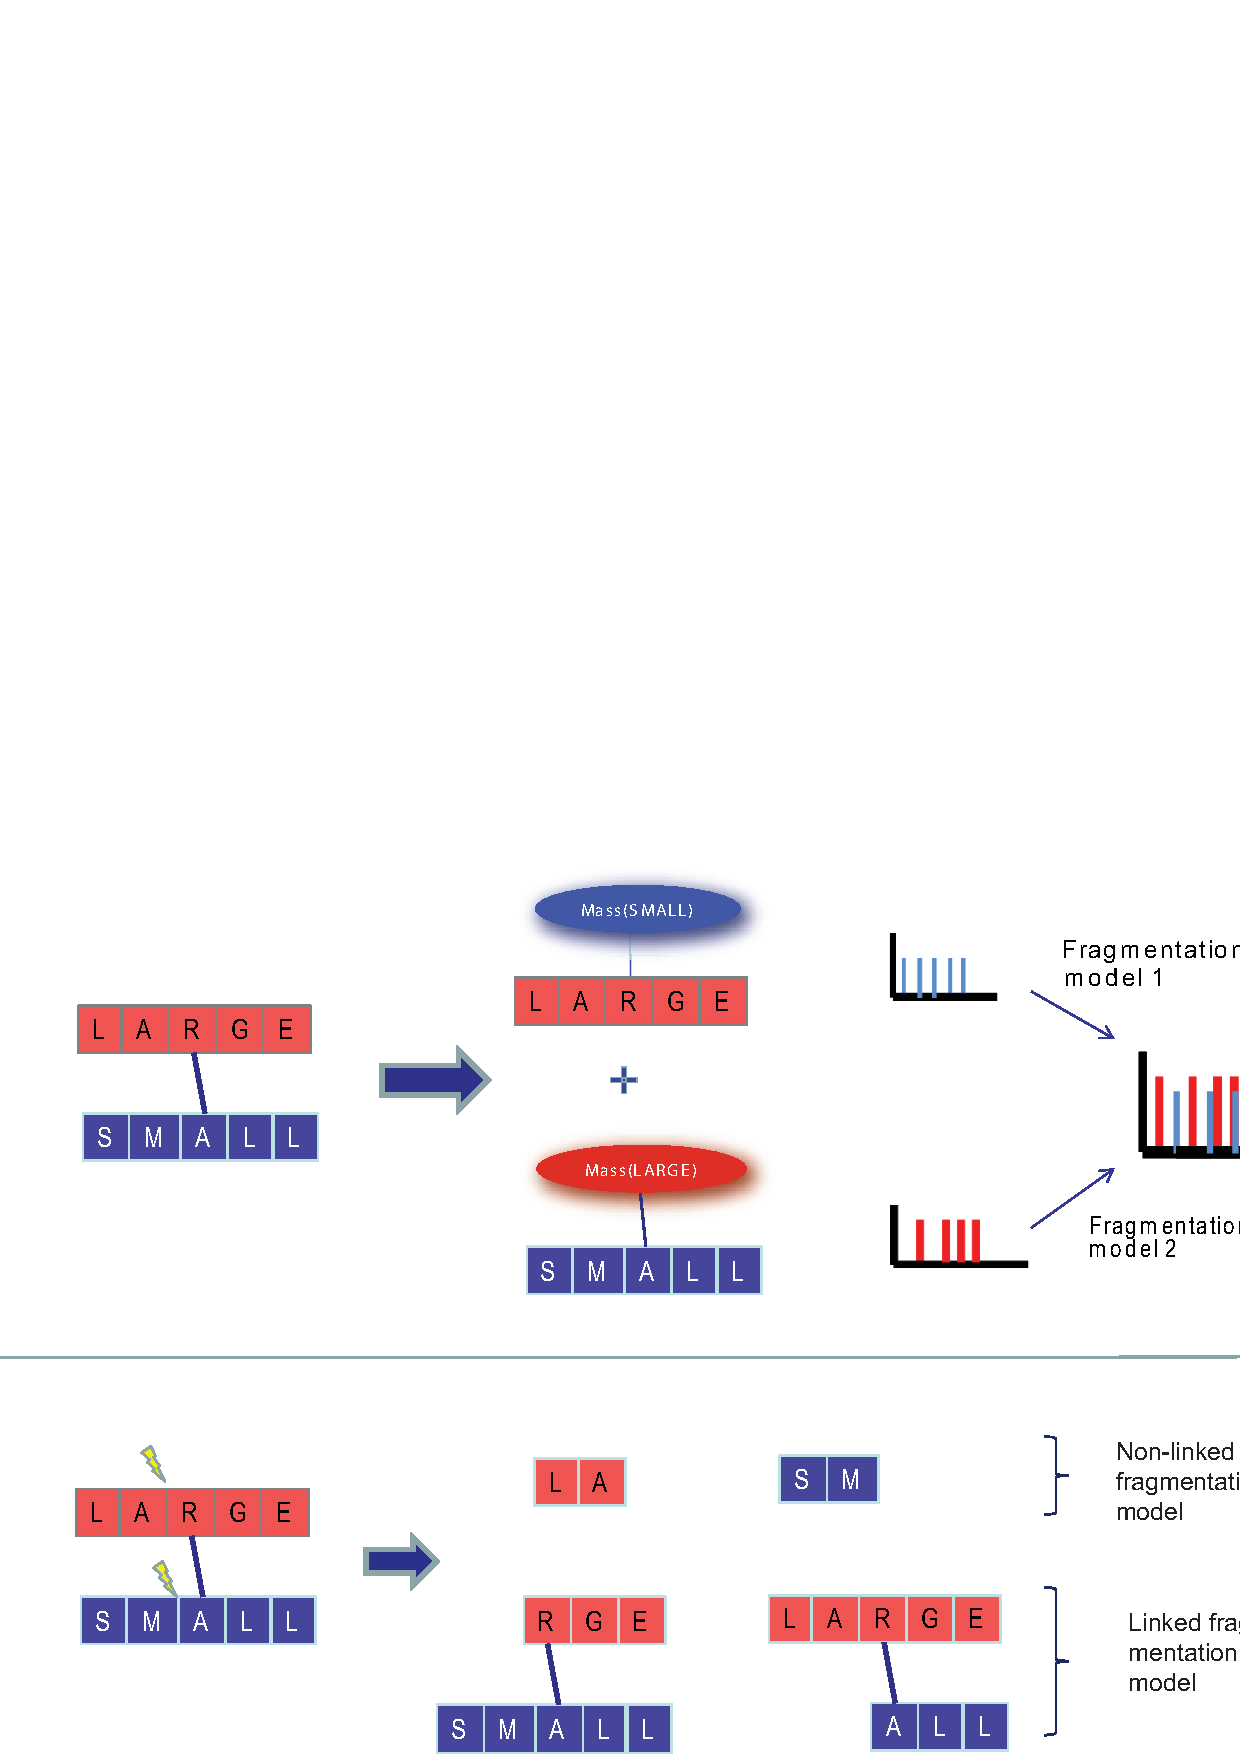
\includegraphics[height=80mm, width=160mm]{TRD4figures/Disulfide_fragment_model.pdf}
		\caption{\footnotesize{\bf Linked peptides fragmentation model.} { {\bf Top panel:} to account for fragment ions from both linked peptides, we model a linked peptide as a mixture of two peptides where each carries a modification with mass equal to the mass of the other peptide plus the mass of the linker (which can possibly be negative, as is the case for disulfide bonds). To generate a theoretical spectrum for a linked peptide pair, our probabilistic model generates a theoretical spectrum for each peptide in the pair and then combines them into the theoretical spectrum for the linked peptide pair. This allows for separate modeling of each linked peptide and can thus capture statistical differences in fragmentation patterns (e.g., when one peptide is long and the other is short). {\bf Bottom panel}: to better capture the specific fragmentation properties of linked peptides, our model separates fragment ions from linked peptides into two categories: linked-fragments and non-linked fragments. Linked fragments are peptide fragments that are covalently linked to a second peptide.  While the fragmentation statistics for non-linked fragments should share some similarity to those of linear peptides, linked-fragments have substantially different fragmentation statistics. In particular we expect higher-charge fragments to be more prominent because linked-fragments carry a second peptide and thus may have an extra N-termini and C-termini tryptic residue to attract charges. Thus in our probabilistic models for linked peptides, all theoretical fragment ions are separated into linked and unlinked fragments, each with separately estimated ion fragmentation statistics.}}
\label{linkedmodel}
\end{figure}

Linked peptides can also arise from various experimental protocols designed to covalently hold proteins together. For example, chemical crosslinking has been shown to be a powerful tool to study protein-protein interactions~\cite{unv}{Sinz06,stengel2012joining,herzog2012structural}.  
%and to help elucidate the structure of large protein complexes
 In such experiments, chemical crosslinkers are added to the samples so pairs of reactive amino acid residues that are spatially close become covalently linked to one another.  Subsequent detection of these linked residues can provide structural information about protein structure and interactions. When the linked residues are from the same protein (intra-protein crosslink), they provide distance constraints to analyze the protein structure. On the other hand, when the linked residues come from different proteins (inter-protein crosslink) they provide evidence that two proteins are in physical contact.

Despite the importance of linked peptides, 
% to help us understand the function, structure and interactions of proteins, 
computational tools to identify them are still in their infancy.  There are three major computational challenges in  identification of linked peptides.
%
First, the covalent linkage of two peptides changes the physicochemical properties of the peptides and thus generates new types of fragment ions which display substantially different fragmentation statistics than those captured by existing models for linear peptides.
%
Second, while spectra from linked peptides contain fragment ions from \emph{two} peptides, almost all MS/MS database search tools 
 assume that each spectrum comes from a single peptide. The presence of two peptides in the same spectrum also creates a quadratic search space for peptide candidates.
% where the number of linked-peptide candidates is in the order of $10^{8}-10^{11}$. 
Efficient techniques are thus needed to efficiently search this vast search space.
%
Third,  there is a small  number of reliably identified publicly available spectra to learn the fragmentation models for linked peptides, thus making the development of these tools quite difficult. This situation is not easily amended because without efficient computational tools to identify MS/MS spectra from linked peptides in the first place, it is almost impossible to construct a large annotated training dataset for linked peptides, a ``chicken-and-egg'' problem.  We aim to break this vicious cycle and to develop a universal tool for identifying linked peptides.

% Extended introduction

\section{Innovation} 

\subsection{Innovation in peptide identification} 

UniQuest will address the following limitations of most peptide identification tools (including MS-GF~\cite{unv}{Kim:2008p5804,Kim:2010p13586}):
inability to estimate E-values accurately for PSMs formed by modified peptides and
limited ability to take advantage of accurate m/z values in  high-precision MS/MS spectra.
%in a variety of ways. MS-GF/MS-GFDB showed promising results for various types of spectra, but they have several  limitations:
%\begin{itemize}
%\item limited support of search for modified peptides including phosphorylated peptides;
%\item inability to compute accurate E-values for PSMs formed by modified peptides
%\item inability to take advantage of accurate m/z values in  high-precision MS/MS spectra;
%\item lack of user-friendly interface;
%\item large running time caused by inefficient preprocessing of the protein database and lack of multithreading support
%\end{itemize}
In addition, it will greatly reduce the  running time by  turning the traditional ``{\em Spectra against Peptides}''  searches into ``{\em Peptides against Spectra}'' searches 
% (as compared to MS-GFDB; 
(see Figure~\ref{DBSearchFig}). 
The advantage of this approach is that it allows one to use the {\em suffix arrays}~\cite{unv}{Manber:1990p15271}, a powerful combinatorial pattern matching technique.  
 UniQuest will also feature an improved usability
due to ProteoSAFe, a user-frendly interface for searches, reports and data management~\cite{unv}{Huang13}. 
%UniQuest will support the HUPO Proteomics Standard Initiative standard file formats~\cite{unv}{Jones:2012p15548}.

The key innovation in designing the precision-aware scoring is a new generative model that describes how a peptide generates a spectrum. 
Kim et al., 2009~\cite{unv}{kim09} introduced an abstract model 
that described a probabilistic process of transforming a Boolean string (peptide) into another Boolean string (spectrum). This simple model was further extended to real spectra and proved to be valuable for designing MS-GF peptide identification tool. 
However, this model, while adequate for low-precision spectra, needs to be modified for high-precision spectra.
UniQuest models a peptide as a boolean string (as before) but model a spectrum as a directed acyclic graph (DAG) called 
{\em $G$-spectrum}  and further applies a transformation of a Boolean string into a $G$-spectrum for scoring real PSMs.
In this G-spectrum representation, 
%vertex and edge labels encode the information on the {\em intensities} and {\em errors} of the peaks
vertex labels encode the information on the {\em intensities} of individual peaks,
and the edge labels encode the information on the {\em mass errors} of pairs of peaks assuming they represent consecutive peaks of the same ion type.
%Note that edge labels are independent on peak intensities.

%The key advantage of MS-GF+ over existing approaches is its ability to compute rigorous E-values (using the generating function %approach~\cite{unv}{Kim:2008p5804})
%and thus to boost the number of peptide identifications.
%While the generating function approach from~\cite{unv}{Kim:2008p5804} worked well in a variety of %studies~\cite{unv}{Zhou:2012p15879,Dresang:2011p15878,Wang:2012p15876},
%the question of applying it to modified peptides and to high-precision MS/MS spectra remained open.

\begin{figure}[tbp]
\begin{center}
\subfigure[]{\includegraphics[width=10cm]{TRD4figures/DBSearch_MSGFDB.pdf}}
\subfigure[]{\includegraphics[width=10cm]{TRD4figures/DBSearch_MSGFPlus.pdf}}
\caption{\footnotesize 
Two approaches for comparing spectra against a protein database.
(a) Traditional {\em Spectra against Peptides} approach compares each spectrum against all peptides. 
(b) UniQuest uses the suffix array and {\em Peptides against Spectra} approach to compare each peptide against all spectra with the same precursor mass.
}
\label{DBSearchFig}
\end{center}
\end{figure}

\subsection{Innovation in peptide sequencing} 

UniNovo will represent the first universal {\em de novo} peptide sequencing tool that will work across {\em all} {\em spectral types} (e.g., the combination of the fragmentation method, the instrument type, and the protease used to digest sample proteins). The scoring function of UniNovo will be easily trainable using a small training dataset consisting of a few thousands of annotated spectra (PSMs). All information needed for {\em de novo} sequencing will be learned from the training dataset. 



%We also present a new representation of  spectrum, the {\em  spectrum logo}, an analog of the sequence logo~\cite{unv}{schneider90} for MS/MS spectrum. Given a spectrum, UniNovo assigns predicted probabilities to each peak  that the peak represents specific ion types (e.g., $y$- or $b$-ions in CID spectrum). In case of the sequence logo, the height of each position (of the sequence alignment) represents the information content of the position (in bits), and the portion of each color encodes the frequency of each of different residues (i.e., nucleotides or amino acids). In the  spectrum logo, the height of each peak represents the information content of the peak (in bits), and the portion of each color encodes the predicted probability of each of different ion types. We show that the  spectrum logo reveals the significant peaks in the spectrum and represents information about their predicted ion types efficiently.





%UniNovo automatically learns all the necessary features (of peaks in the spectrum) from the training dataset. Each feature in UniNovo considers not only the intensity of a peak but also the relation between peaks in the spectrum, allowing UniNovo to efficiently capture the characteristics of various fragmentation methods.  Based on the features of peaks, UniNovo estimates the probabilities that each peak is from selected ion types (e.g., $y$- or $b$-ion types). The estimation results of peaks are then used to construct the spectrum graph, on which candidate {\em de novo} sequences are efficiently selected using a dynamic programming algorithm~\cite{unv}{dancik99,chen01}. 

One of the biggest challenges in  {\em de novo} sequencing is to estimate the error rate of the resulting  {\em de novo} reconstructions.  
%Unlike peptide identification tools 
%that commonly uses the {\em target-decoy approach}~\cite{unv}{elias07,nesvizhskii10} to estimate the statistical significance of the %peptide identifications, 
%{\em de novo} peptide sequencing tools have rarely been subjected to a statistical significance analysis in the past. 
Several {\em de novo} sequencing tools report the error rate of amino acid predictions (e.g. confidence scores in PEAKS), but this is often not sufficient because the overall quality of the sequence cannot be easily determined by the error rates of individual amino acid predictions. 
%
Estimating the probability that the entire reconstructed peptide (rather than individual amino acids) is correct is crucially important for downstream applications (e.g., blind database search) since a single error in the reconstruction may lead to a failure of such an application. 

To our knowledge, only PepNovo+~\cite{unv}{frank09}, developed at CCMS,  reports the empirical probability that the output peptide is correct.
% (using logistic regression with multiple features of the reconstructions). 
% such as length and score, which are extracted from a training dataset consisting of hundreds of thousands of annotated %spectra
However,  PepNovo+ does not include an automated training procedure (that would allow to easily extend PepNovo+ for newly emerging MS approaches) and is currently trained only for CID. Since PepNovo+ was not originally designed as a universal tool, extending PepNovo+ beyond CID spectra requires training complex boosting-based models for predicting peak ranks and rescoring peptide candidates. Moreover, PepNovo+ training includes several manual steps and requires large corpus of training spectra (a few hundred thousands of PSMs).  Thus,   in case of non-CID fragmentation methods, it remains unclear how to obtain accurate error rate estimation for {\em de novo} reconstructions using PepNovo. We thus decided to develop a new universal tool UniNovo rather than to extend PepNovo into a truly universal tool. 
%UniNovo will estimate  the probability that each reported reconstruction is correct, using simple statistics that are readily %obtained from a small training dataset. 

\subsection{Innovation in identification of linked peptides} 

We propose new probabilistic scoring model that captures the fragmentation characteristics of linked peptides.  A linked peptide spectrum is modeled as a spectrum from a pair of peptides in order to account for all  possible fragment ions from both peptides (Figure~\ref{linkedmodel}a) and the proposed models explicitly address the co-fragmentation of a pair of peptides to score a LinkedPeptide-Spectrum Match (LPSM).  
%This framework also allow us to build separate scoring model for each of the linked peptides, accounting for their difference in fragmentation statistics. 
Our proposed model further separates fragment ions into linked and unlinked fragments to model the highly-charged fragment ions that are specific to linked peptides (Figure~\ref{linkedmodel}b).  With this new model we derive a filtration strategy based on the concept of vector projection to filter the search space of all possible peptide pairs by several order of magnitude.  Finally in order to obtain a training dataset we utilize combinatorial peptide synthesis to generate a large set of linked peptides and couple it with a search strategy that takes advantage of the special design of the peptide library to identify MS/MS spectra from these linked peptides.

\section{Approach}

\subsection{Aim 1: Peptide identification} 

UniQuest  takes a spectral dataset $Spectra$  and a protein database $ProteinDB$ as an input and
outputs a set of scored PSMs along with statistical significance estimates.
%\footnote{$ProteinDB$ can be regarded as a long string generated by concatenating all protein sequences (with %delimiters).}
The workflow of MS-GF+ comprises
the following 4 steps: generating spectral vectors, searching a protein database, 
computing E-values of PSMs, and estimating FDRs. 


To make UniQuest statistically sound, we adopt the generating function approach 
 to rigorously compute E-values of PSMs using the score distribution of \emph{all peptides}~\cite{unv}{Kim:2008p5804}.
  The scores of PSMs reported by existing peptide identification tools are often poorly
correlated with their statistical significance (e.g., E-values)~\cite{unv}{Granholm:2011p15084}.  
It is important to rank PSMs based on their statistical significance,
because such ranking  (rather than ranking based on ``raw scores'')
often dramatically increases the number of identified spectra~\cite{unv}{Kim:2008p5804,Klammer:2009p13118}.
This observation explains why it is important to make UniQuest statistically sound (condition (c)).
%Many database search tools
%estimate an E-value of a PSM based on an approximation of
%a tail of the score distribution specific to the spectrum using \emph{peptides
%in the database}~\cite{unv}{Geer:2004p1847,Craig:2004p5582,Klammer:2009p13118}.
%Since this approach is known to result in biased estimates of statistical significance~\cite{unv}{Kim:2008p5804}, 
%we will adopt the generating function approach to rigorously compute E-values of PSMs using the score distribution of \emph{all %peptides}~\cite{unv}{Kim:2008p5804}.
The spectral vector scoring model described below is essential here, because the generating function approach is easily applicable to the scoring functions that can be represented as a dot-product of vectors~\cite{unv}{Gupta:2011p15442}.
%Adopting the generating function approach in UniQuest (and extending it to modified peptide and high-accuracy spectra) will improve the accuracy of E-%value estimates and increase the number of identified peptides. 


Below we describe
each step and explain how to address the challenge of implementing universal as well as modification-aware and precision-aware MS/MS database search tool.
% while enforcing the unversal condition for the scoring function.  
% assuming that the parameters required to convert a spectrum into a PRM spectrum has been already trained as described in Kim et al.~\cite{unv}{Kim:2010p13586}

\subsubsection{Generating spectral vectors}

\paragraph{Rescaling mass values}

A spectral vector~\cite{unv}{Kim:2010p13586,Tanner:2005p2048} of a spectrum $S$ is an $M$-dimensional vector with integer values where $M$ is the nominal parent mass of $S$. 
%We denote the nominal parent mass of $S$ as $\textrm{ParentMass}(S)$.
Transformation of experimental spectra into spectral vectors requires {\em binning}.
To support this transformation, the generating function approach was designed under the assumption that amino acid masses are integers.
%MS-GF used nominal masses as integer masses of amino acids.
While this enables efficient computing of scores, 
it causes rounding errors because peaks in the spectrum correspond to {\em real} rather than {\em nominal} masses of amino acid sequences.
To minimize the rounding errors, we {\em rescale} every mass $m$ into $0.9995m$~\cite{unv}{kim09,Taylor:1997p9273,Bern:2007p7752}.
%This rescaling minimizes the difference between nominal masses and (rescale masses of single amino acids and even of peptides . 
This dramatically reduces the rounding errors,
% (Table~\ref{RescalingTable}), 
so one can estimate the nominal mass of a peptide (or a peak) of mass $m$ by simply taking $[0.9995m]$ where $[x]$ represents the closest integer to $x$.
%For example, for a peptide ``RESCAILINGMASSES'' of mass 1705.776, $[1705.776 \cdot 0.9995=1704.92]=1705$ represents the correct nominal %mass of the peptide.
We investigated all 188 million unique peptides of length up to 20 in the human IPI database 
%(version 3.87), 
and the estimation was inaccurate only for 874 peptides ($4.6 \times 10^{-6}$ \%).
%The percentage only increases to 0.07\% for peptides of lengths up to 40. 




\paragraph{Transforming spectra into spectral vectors}
\label{PRMGen}

%Many database search tools convert a peptide into a ``theoretical'' spectrum and compare it with an experimental spectrum using scoring functions of %various complexity.
%UniQuest  converts spectra into \emph{spectral vectors}~\cite{unv}{Kim:2010p13586,Tanner:2005p2048}. 
%Using dot-product for scoring has  advantages since it is currently the only scoring function  enabling computing rigorous p-values of %PSMs~cite{Gupta11}.

The conversion from an experimental spectrum to a spectral vector proceeds as follows.
A \emph{spectrum} $S=\{(mz_1,rank_1),\ldots,(mz_l,rank_l)\}$ is represented as a set of {\em ranked} peaks where the $i$th highest intensity peak gets rank $i$
($mz_j$ and $rank_j$ represent m/z and rank of $j$th peak, respectively).
An \emph{ion type} is represented as a triplet of integers {\em charge, offset}, and {\em sign}, where sign represents whether the ion type is a prefix ion ($sign=1)$ or
a suffix ion ($sign=-1$). For example, singly-charged b-ions and y-ions correspond to ion types (1, 1, 1) and (1, 19, -1), respectively.
Given an ion type $ion=(charge,offset,sign)$, one can turn a spectrum $S$ of nominal parent mass $M$ into $S_{ion}=\{(mass_1,rs_1),\ldots,(mass_l,rs_l)\}$ using the following transformation: 
$$
  mass_j = \left\{
    \begin{array}{ll}
      [mz_j \cdot charge \cdot 0.9995]-offset & \textrm{if } sign = 1\\
      M - \big([mz_j \cdot charge \cdot 0.9995]-offset \big) & \textrm{if } sign = -1
    \end{array} \right.
$$
$$
 rs_j = \mathrm{RankScore}(ion,rank_j),
$$
where $\mathrm{RankScore}(ion,rank)$ is a pre-computed function that takes an ion type $ion$ and an integer $rank$ and returns a
probabilistic log-likelihood score defined in~\cite{unv}{Kim:2010p13586,kim09}. 
%\footnote{In practice, $\mathrm{RankScore}(ion,rank)$ also accounts for the location of
%the observed peak and the precursor charge and mass of the spectrum, which are omitted
%here for simplification. }
Assume that $\mathcal{I}$ is a set of ion types contributing to scoring. 
The spectral vector of $S$ (denoted by $\vec{S}=(s_1, \ldots, s_M$) is computed as follows:
$$
s_i = \sum_{ion \in \mathcal{I}}  \max (\{rs ~|~ (mass,rs) \in S_{ion} \textrm{ and } mass = i \} \cup \textrm{RankScore}(ion,\infty)),
$$
where $\textrm{RankScore}(ion,\infty)$ represents the score given when $ion$ is missing.
%Note that $\mathcal{I}$ and $\mathrm{RankScore}$ are pre-computed from a training set as described in Kim et al.~\cite{unv}{Kim:2010p13586}.

\paragraph{From peptides to peptide vectors}

 A (non-modified) \emph{peptide} is defined as a string over the alphabet  $\mathcal{A}$ of 20 standard amino acids. UniQuest is a restrictive MS/MS database search tool that allows a user to specify a set of allowed modifications.
Let $\mathcal{A}^+$ be an {\em extended} amino acid set containing both unmodified and modified amino acids.
For an (unmodified) amino acid $a\in\mathcal{{A}}$, let $\textrm{Mod}(a) \subset \mathcal{A}^+$ be the \emph{set} of both unmodified and modified amino acids associated with $a$. 
For example, if $T$ (Thr) and $T^*$ (phosphorylated Thr) are in $\mathcal{A}^+$, $\textrm{Mod}(T)=\{T, T^*\}$.
%If $a$ can be modified, $|\mathrm{Mass}(a)|>1$ (e.g. if Met can be oxidized, $\mathrm{Mass}(M)=\{131,147\}$), and otherwise $|\mathrm{Mass}(a)|=1$. 
Given a peptide $P=a_{1}\ldots a_{k}$, define $PV=pv_{1} \ldots pv_{k}$ as a \emph{variant} of $P$
if $pv_{i}\in\mathrm{Mod}(a_{i})$ for all $i$ ($1\leq i\leq k$).
%Below we abbreviate the peptide variant as {\em variant}.

We  define a peptide vector of a variant as follows.
Let $\textrm{Mass}(a)$ be the nominal mass of a (possibly modified) amino acid $a$.
For example, $\textrm{Mass}(T)=101$ and the mass of phosphorylated Thr is $\textrm{Mass}(T^*)=181$.
Given a variant $PV=pv_{1}\ldots pv_{k}$, define the mass of $PV$ as $\textrm{Mass}(PV)=\sum_{i=1}^{k}\textrm{Mass}(pv_{i})$.
Given a variant $PV=pv_{1}\ldots pv_{k}$ of mass $M$, we define its peptide vector (denoted
by $\vec{PV}$) as a 0-1 vector $(m_{1}, \ldots,  m_{M})$
with $(n-1)$ 1s, such that $m_{i}=1$ if $i$ equals to 
$\textrm{Mass}(pv_{1})+\ldots+{Mass}(pv_{j})$ $(1\leq j \leq k)$.


%\subsubsection{Removing precursor-related peaks}

%Some types of spectra (e.g., ETD spectra) often feature high-intensity precursor
%peaks, charge-reduced precursor peaks, and their neutral and side-chain
%losses. While these peaks are not informative,
%they may artificially inflate scores of false PSMs if they fall in the positions of certain ion types.
%UniQuest removes
%precursor-related peaks prior to generating spectral vectors to eliminate a risk of erroneously interpreting them as other ion
%types. The information on which peaks to remove is automatically pre-computed from a training set~\cite{unv}{Kim:2010p13586}.

%\subsubsection{Scoring a peptide-spectrum match}

 Score  of
a PSM $(PV,S)$ is defined as $\mathrm{MSGFScore}(PV,S)=\vec{PV} \cdot \vec{S}$
   if $\textrm{Mass}(PV) = \textrm{ParentMass}(S)$
and $-\infty$ otherwise. The score represents the log likelihood
ratio described in~\cite{unv}{kim09}.
%of the probability that $S$ is generated from $V$ over the probability that $S$ is generated from a random variant~\cite{unv}{kim09}. 


%Given $\vec{S}=s_{1}\ldots s_{M}$,
%let $\mathrm{MaxScore}(i)$ be the maximum score of a variant of mass $i$
%against $s_{i}\ldots s_{i}$. $\mathrm{MaxScore}(i)$ can be calculated
%as follows:
%
%\[
%\mathrm{MaxScore}(i)=\max_{\mbox{a \ensuremath{\in\mathcal{A}}}}\max_{m\in Mass(a)}\left\{ \mathrm{MaxScore}(i-m)+s_{i}\right\} .
%\]
%We initialize $\mathrm{MaxScore}(0)=0$ and $\textrm{\ensuremath{\mathrm{MaxScore}(i)=0}}$
%for negative $i$. Then, $\mathrm{MaxScore(M)}$ represents the de
%novo sequencing score.

\subsubsection{Searching a protein database with suffix arrays}
\label{sec:DBSearch}

We define $ProteinDB^+$ as the set of all variants (with respect to an extended amino acid set $\mathcal{A}^+$) derived from $ProteinDB$.
We aim to solve the following problem: given a spectral dataset $Spectra$ and a protein database $ProteinDB$, for each spectrum $S \in Spectra$ find a variant $PV_{S,ProteinDB}$ such that
$$
PV_{S,ProteinDB} = \operatorname*{arg\,max}_{PV \in ProteinDB^+} \textrm{MSGFScore}(PV,S).
$$

\noindent Solving this problem involves the following three steps: 
(1) for every spectrum $S \in Spectra$, computing $\vec{S}$, 
(2) for every variant $PV \in ProteinDB^+$, computing $\vec{PV}$, 
and (3) for every pair of $(PV,S)$ where $\textrm{Mass}(PV)=\textrm{ParentMass}(S)$, computing $\mathrm{MSGFScore}(PV,S)=\vec{PV} \cdot \vec{S}$. 
To execute these steps efficiently, one may simply execute the step (1) and (2), store all $\vec{S}$ and $\vec{PV}$ in the main memory and execute the step (3).
But this is often infeasible because the number of variants is usually too large to fit all $\vec{PV}$ in the main memory.
Alternatively, one may consider executing the step (2) on the spot for each spectrum, but this is prohibitively slow.%
%\footnote{For the IPI human database, executing the step (2) alone takes 54 seconds, considering partially tryptic peptides %of lengths between 6 and 40, and two variable modifications Oxidation of Met and protein N-term Acetylation.}

Instead of storing both $\vec{S}$ and $\vec{PV}$, we propose to store only $\vec{S}$ for all spectra in the main memory, and 
index them by parent masses. 
Since spectral vectors compactly represent experimental spectra, they can be stored in a memory-efficient manner (4GB per 200,000 spectra). 
Rather than finding the best scoring peptide for each spectrum, we propose to find the best scoring spectrum for each variant.
%
For each variant $PV \in ProteinDB^+$, UniQuest finds a spectrum $S_{PV,Spectra}$ such that
%Since $\textrm{MSGFScore}(V,S)=-\infty$ if $\textrm{Mass}(V) \neq \textrm{PrecursorMass}(S)$, the above equation can be rewritten as follows:
\begin{equation}
\label{DBSearchProblem}S_{PV,Spectra} = \operatorname*{arg\,max}_{S \in Spectra} \textrm{MSGFScore}(PV,S)
= \operatorname*{arg\,max}_{S \in Spectra_{\textrm{Mass}(PV)}} \textrm{MSGFScore}(PV,S),
\end{equation}
where $Spectra_{\textrm{Mass}(PV)}$ represents the set of spectra $S \in Spectra$ with $\textrm{ParentMass}(S) = \textrm{Mass}(PV)$.
This problem can be solved efficiently by enumerating variants $PV \in ProteinDB^+$ one by one, generating $\vec{PV}$ {\em on the spot},
and computing $\textrm{MSGFScore}(PV,S)=\vec{PV} \cdot \vec{S}$ for all {\em pre-computed} $\vec{S}$ where $S \in S_{\textrm{Mass}(PV)}$.
%Once $S_{PV,Spectra}$ is found for all variants $PV$, finding $PV_{S,ProteinDB}$ is trivial because 
%$PV_{S,ProteinDB} = \operatorname*{arg\,max}_{PV \in \{PV | S_{PV,Spectra} = S, PV \in ProteinDB\}} \textrm{MSGFScore}(PV,S)$.

%In practice, to save the memory, instead of recording $S_{PV,Spectra}$ for every $PV$,
%while enumerating variants, 
%MS-GF+ records the best scoring variant $PV^*$ while enumerating PVs,
%and updates $PV^*$ to $PV$ whenever it finds $PV$ where $S_{PV,Spectra} = S$ and $\textrm{MSGFScore}(PV,S) > %\textrm{MSGFScore}(PV^*,S)$. 

Similar to pFind~\cite{unv}{Zhou:2010p14814}, we will use a {\em suffix array}~\cite{unv}{Manber:1990p15271} of $ProteinDB$
% (a lexicographically sorted list of all the suffixes of $ProteinDB$~\cite{unv}{Manber:1990p15271}) 
to further optimize the database search. 
%
%Protein databases (particularly, eukaryotic ones)
%contain many similar proteins, so many peptides appear in multiple
%copies in a database (\emph{repeated peptides}). For example,
%the IPI human database (version 3.87) contains about 130,000 fully-tryptic
%peptides of length 10, but the number decreases to about 50,000 if
%only unique peptides are considered. 
%
%If a protein database is indexed as a suffix array, peptide occurrences from the same repeated  peptide
%appear in neighboring indices in the suffix array. 
Instead of
searching peptides according to their ordering in the original database
file, UniQuest will search peptides according to their ordering in the
suffix array, and use the longest common prefix data structure~\cite{unv}{Manber:1990p15271}
to score each unique peptide only once (Figure~\ref{DBSearchFig} (b)). 


\subsubsection{Designing modification-aware scoring}
\label{sec:EValue}

While Kim et al., 2008~\cite{unv}{Kim:2008p5804} described the  generating function algorithm for computing {\em exact} p-values in the case of unmodified peptides, it is unclear how to extend this approach to modified peptides. 

Given a spectrum $S$, a score threshold $t$, an extended set of amino acids $\mathcal{A}^+$, and a database size $N$, we define E-value$(S,t,\mathcal{A}^+,N)$ as the expected number of variants  $PV$ 
%(as defined by $\mathcal{A}^+$) 
with $\mathrm{MSGFScore}(PV,S) \geq t$
 in a random protein database of size $N$.
% \footnote{The random database assumes that the probability of finding a peptide $P$ starting in an arbitrary position of the database equals to $\mathrm{Prob}(P)$.%}  
To compute E-value$(S,t,\mathcal{A}^+,N)$, we first compute {\em spectral E-value} E-value$(S,t,\mathcal{A}^+)$, the expected number of variants $PV$ with $\mathrm{MSGFScore}(PV,S) \geq t$ given a {\em single random peptide}.
A single random peptide models a random peptide starting at a fixed position in a random protein database.

We consider a set of all possible (unmodified) peptides of length $k$ (where $k$ is a large number) and 
select a random peptide uniformly from this set (i.e. the probability of selecting a peptide is $\frac{1}{20^k}$).
%\footnote{In practice, to reflect different frequencies of amino acids in a database (e.g. Leu is usually more common than Trp), we define the %probability of a peptide $P=a_1 \ldots a_k$ as $\prod_{i=1}^{k} \textrm{Prob}(a_i)$ where \textrm{Prob}(a) is the frequency of amino acid $a$ in %a protein database. 
%Note that this does not change the algorithm to compute spectral E-values.}
%We say that a peptide (of length $k$) {\em fits} a spectrum if a variant of a prefix of this peptide has a nominal mass equal to the nominal precursor mass of the spectrum~\cite{unv}{Gupta:2011p14505}.
We say that a peptide $P$ {\em produces} a variant $PV$ if $PV$ is a variant of a prefix of $P$.
For example, $PEPT^*$ and $PEPTI$ are produced by $PEPTIDE$.
Given a spectrum $S$, let $\mathcal{PV}(t)$ be the set of all variants $PV$ with $\textrm{MSGFScore}(PV,S) \geq t$.
%Each variant $V \in \mathcal{PV}(t)$ appears in $20^{k-|V|}$ random peptides of length $k$. 
For every variant $PV$, there are $20^{k-|PV|}$ peptides of length $k$ producing a variant $PV$ ($|PV|$ stands for the number of amino acids in $PV$).
Therefore, expected number of variants per random peptide with a score equal or better than $t$ is
$$
\textrm{E-value}(S,\mathcal{A}^+,t) = \sum_{PV \in \mathcal{PV}(t)}  \frac{20^{k-|PV|}}{20^k} = \sum_{PV \in \mathcal{PV}(t)} 20^{-|PV|}.
$$
Since a variant is a string over the alphabet $\mathcal{A}^+$, this expression can be computed using the generating function approach~\cite{unv}{Kim:2008p5804}.
Given a spectrum $S$ with $\vec{S} = s_1 \ldots s_M$, consider an {\em amino acid graph} $G(V,E,\mathcal{A}^+)$ with $V=\{0,\ldots,M\}$ and $E=\{(i,j) | j-i \in \textrm{Mass}(a) \textrm{ for } a \in \mathcal{A}^+\}$, where the {\em score} of a vertex $i$ is defined as $s_i$, the {\em probability} of an edge is defined as $\frac{1}{20}$, the score of a path is defined as the sum of scores of its vertices, and the {\em probability} of a path is defined as the product of probabilities of its edges.
A path in an amino acid graph represents a variant.
Therefore, $\textrm{E-value}(S,\mathcal{A}^+,t)$ equals to the sum of probabilities of all paths from 0 to $M$ with scores equal or better than $t$, and can be computed using parametric dynamic programming~\cite{unv}{Kim:2008p5804,kim09}.

While spectral E-values are useful for evaluating statistical significance of
individual
 PSMs (independently of the database), they need to be transformed into  $\textrm{E-value}(S,t,\mathcal{A}^+,N)$
to take
into account the fact that the database search represents ``multiple testing''~\cite{unv}{Noble:2009p13095}.
% where multiple variants (arising from different database peptides) are scored against a spectrum
%Given a variant $V$, a spectrum $S$, and a database of size $N$, the
%database E-value of $V$ and $S$ (denoted by $\mathrm{DatabaseEValue}(V,S)$
%can be approximated as follows:
E-values can be approximated as follows:
$$
\textrm{E-value}(S,t,\mathcal{A}^+,N) \approx \textrm{E-Value}(S,t,\mathcal{A}^+) \cdot N,
$$
\noindent where $N$ is the size of the database.% 
%\footnote{Since protein databases contain many repeated peptides in practice, it is important to reflect an {\em effective} %size of the database that is estimated as the number of unique peptides of certain length.}

%denotes the number of \emph{unique peptides}
%in the database whose length equals to the length of $V$. The number
%of unique peptides in a database can be efficiently computed using
%the LCP information of a suffix array of the database.
%
%{\tt The text in the last paragraph needs to be redone based on a new formulation for
%E-values.}


Existing MS/MS database search tools output a set of PSMs and estimate the FDR of this set 
%(fraction of erroneous PSMs)
 using the {\em Target-Decoy Approach} (TDA).  
In addition to computing the FDR via TDA, our approach 
also provide a possibility to estimate the FDR via E-values of PSMs
% (denoted by Expected FDR or EFDR) 
without using TDA~\cite{unv}{Gupta:2011p15442}.
%also supports computing FDRs using database E-values (denoted by expected FDR or EFDR) 
%without searching the decoy database as described in~\cite{unv}{Noble:2009p13095,Gupta:2011p14505}. 
While using TDA to computing FDR for {\em each type} of modification encountered in the search remains an open problem, our E-value based approach seamlessly addresses this problem.   



\subsubsection{Designing precision-aware scoring}

\paragraph{Extending the generating function approach to high-precision spectra} 

Mass spectrometers are usually divided into High-precision (denoted by H) and Low-precision (denoted by L) instruments.
Depending on whether the precursor and product ions are measured with Low or High-precision, the spectra are divided into LL, LH, HL, and HH spectra (LH spectra are hardly ever used in proteomics).

The key part of the generating function approach is the assumption that amino acids have integer masses~\cite{unv}{Kim:2008p5804}. However, rounding amino acid masses into integers introduces  errors.
These rounding errors reduce after rescaling by 0.9995 
%as described in~\cite{unv}{kim09,Taylor:1997p9273,Bern:2007p7752}, 
making them appropriate for  LL and HL spectra.
However, for HH spectra, the rounding errors remain too large even after rescaling,
prohibiting UniQuest  from benefiting from precise product ion peaks. A possible
solution to this problem is to change the constant used
for rescaling. For example, for a scaling constant 274.335215,  
%(e.g. $\mathrm{mass}(G)=57.021464 \times 274.335215=15642.995586\approx15643$),
the rounding error is bounded by 2.5 ppm, which is appropriate for analyzing
HH spectra. However, since the time complexity of the generating function
algorithm is proportional to 1 over the rescaling constant, this makes
computing E-values prohibitively slow.
UniQuest will use a new scoring algorithm taking advantage of accurate product ion masses while not substantially increasing the running
time. 

%Mass spectrometers are usually divided into High-precision (denoted by H) and Low-precision (denoted by L) instruments.
%Depending on whether the precursor and product ions are measured with Low or High-precision, the spectra are divided into LL, LH, HL, and HH %spectra (LH spectra are hardly ever used in proteomics studies).
%While it may appear that extending the generating function approach from LL (as defined in~\cite{unv}{Kim:2008p5804}) to HL and HH spectra is a simple %matter of tuning parameters that control the error tolerance,
%the situation is more complex. 
%Here we explain how to take advantage of high-precision product ion peaks.

\paragraph{Database search of high-precision spectra}

Let $\textrm{RMass}(a)$ be the real mass of an amino acid $a$.
For a variant $PV=pv_1 \ldots pv_k$, let $\textrm{RMass}(PV) = \sum_{i=1}^{k}\textrm{RMass}(pv_i)$, and $\textrm{RParentMass}(S)$ be the real parent mass of a spectrum $S$.
We previously defined $\mathrm{MSGFScore}(PV,S)=\vec{PV} \cdot \vec{S}$ if $\textrm{Mass}(PV) = \textrm{ParentMass}(S)$
and $-\infty$ otherwise.
Note that the condition $\textrm{Mass}(PV) = \textrm{ParentMass}(S)$ while appropriate for LL spectra is weak for HL and HH spectra,
because it may be satisfied even when real mass $\textrm{RMass}(PV)$ significantly deviates (e.g. up to 0.5 Da) from $\textrm{RParentMass}(S)$. 
To take advantage of accurate parent masses in HL and HH spectra, this condition has to be redefined to 
$\textrm{RMass}(PV)-\Delta < \textrm{RParentMass}(S) < \textrm{RMass}(PV) + \Delta$, where $\Delta$ is the precursor mass tolerance.
To solve the database search problem for this modified definition of $\textrm{MSGFScore}$, 
the equation~\ref{DBSearchProblem} should be changed as follows:

\begin{equation}
\label{ModDBSearchProblem}
S_{PV,Spectra} = \operatorname*{arg\,max}_{S \in Spectra} \textrm{MSGFScore}(PV,S)
= \operatorname*{arg\,max}_{S \in Spectra_{\textrm{RMass}(PV)}} \textrm{MSGFScore}(PV,S),
\end{equation}
where $Spectra_{\textrm{RMass}(PV)}$ represents the set of spectra $S \in Spectra$ satisfying $\textrm{RMass}(PV)-\Delta < \textrm{RParentMass}(S) < \textrm{RMass}(PV) + \Delta$.

\paragraph{From spectral vectors to $G$-spectra}
\label{sec:ScoringHH}

%The key part of the generating function approach is the assumption that amino acids have integer masses (otherwise the parametric dynamic programming is difficult to implement). However, rounding amino acids to integers introduce rounding errors.
%As mentioned earlier, the rounding error reduces after rescaling by 0.9995, making it appropriate for  LL and HL spectra.
%However, for HH spectra, the rounding error remains too large even after rescaling,
%prohibiting MS-GF+ from benefiting from precise product ion peaks. A possible
%solution to this problem is to change the constant used
%for rescaling. For example, for a scaling constant 274.335215 (e.g. $\mathrm{mass}(G)=57.021464*274.335215=15642.995586\approx15643$),
%the rounding error is bounded by 2.5 parts per million (ppm), which is appropriate for analyzing
%HH spectra. However, since the time complexity of the generating function
%algorithm is proportional to 1 over the rescaling constant, this makes
%computing E-values prohibitively slow.
%
%Here we present a new scoring algorithm taking advantage of accurate
%product ion masses while not substantially increasing the running
%time of MS-GF+. 

Kim et al., 2009~\cite{unv}{kim09} introduced an abstract model 
that described a probabilistic process of transforming a Boolean string (peptide) into another Boolean string (spectrum). This simple model was further extended to real spectra and proved to be valuable for designing MS-GF peptide identification tool. 
However, this model, while adequate for low-precision spectra, needs to be modified for high-precision spectra.
Below, we model a peptide as a boolean string (as before) but model a spectrum as a directed acyclic graph (DAG) called 
{\em spectral DAG} and further apply a transformation of a Boolean string into a spectral DAG for scoring real PSMs.

%%%%%%%%%%%%
%Let $P=p_0 \ldots p_M$ be a Boolean string called a {\em peptide} where $p_0=p_M=1$.
%Let $S=$.
%
%Let $G_{S}=(V,E,\mathcal{A}^+)$ be a directed acyclic graph called a {\em spectrum} with a labeling $l: V \to \{0,1\}$ and an edge labeling $e:E \to \{0,1\}$,
%where the vertex set $V=\{0, \ldots, M \}$, 
%and the edge set $E=\{(i,j) | j-i \in \textrm{Mass}(a) \textrm{ for } a \in \mathcal{A}^+ , v_i=1, v_j=1\}$.
%Let $G_S=(V,E,\mathcal{A}^+)$ be a edge-labeled graph.
%
%$a \ in {\mathcal{A}^+} \cup {0}$, 


%%%%%%%%%%%%%

%The basic idea is to modify the scoring algorithm to utilize the peaks separated by a single  amino acid mass. 
Let $P=p_1 \ldots p_M$ be a Boolean string called a {\em peptide}.
%Let $S=s_1 \ldots s_M$ be a Boolean string called a {\em spectrum}.
Let $G_S=(V,E,\mathcal{A}^+)$ be a labeled DAG called a {\em G-spectrum} with vertices $V=\{0, \ldots, M \}$, and edges $E=\{(i,j) | j-i \in \textrm{Mass}(a) \textrm{ for } a \in \mathcal{A}^+ \}$.
%a vertex labeling $v:V \to \{0,1\}$,and an edge labeling $e:E \to \{0,1\}$.
We define the Boolean label of vertex $i$ as $v_i$ and edge $(i,j)$ as $e_{i,j}$.
The probability of a peptide $P$ generating a G-spectrum $G_S$ is defined as follows:
$$
\textrm{Prob}(G_S|P)=\prod_{i \in V} \textrm{Prob}_{\textrm{V}}(v_i | p_i) \cdot \prod_{(i,j) \in E} \textrm{Prob}_{\textrm{E}}(e_{i,j} | p_i, p_j),
$$
where $\textrm{Prob}_{\textrm{V}}(x|y)$ is a $2 \times 2$ matrix representing the probability of a peptide character (0 or 1) generating a vertex label,
and $\textrm{Prob}_{\textrm{E}}(x|y,z)$ is a $2 \times 4$ matrix representing the probability of a pair of peptide characters generating an edge label (Figure~\ref{ProbTable}).
In practice, $\beta_1 \approx \beta_2 \approx \beta_3$.
% (see Figure~\ref{ProbTable} (b)).

\begin{figure*}[tbp]
\centering
\subfigure[]{
\begin{tabular}[b]{r|cc}
 \backslashbox{$x$}{$y$}& 0 & 1 \\
 \hline
 0 & $\theta$ & $1-\rho$ \\
 1 & $1-\theta$ & $\rho$ \\
 \end{tabular}\hspace{0.2in}
}
\subfigure[]{
\begin{tabular}[b]{r|cccc}
\backslashbox{$x$}{$y,z$}& 0,0 & 0,1 & 1,0 & 1,1 \\
\hline
0 & $\beta_1$ & $\beta_2$ & $\beta_3$ & $1-\alpha$ \\
1 & $1-\beta_1$ & $1-\beta_2$ & $1-\beta_3$ & $\alpha$ \\
\end{tabular}\hspace{0.2in}
}
\caption{\footnotesize \textbf{(a)} Probability $\textrm{Prob}_{\textrm{V}}(x|y)$ of a peptide character
$y$ generating a vertex label $x$. 
\textbf{(b)} Probability $\textrm{Prob}_{\textrm{E}}(x|y,z)$ of peptide characters
$y$ and $z$ generating an edge label $x$. 
}
\label{ProbTable}
\end{figure*}

When applying this model for scoring a peptide $P$ and a G-spectrum $G_S$, we consider a test comparing two hypotheses: 
one assuming $G_S$ is generated by $P$ and the other assuming $G_S$ is generated by a string consisting of all zeros (denoted by $O$).
The score of $(P,G_S)$ (denoted by $\textrm{Score}(P,G_S)$) is defined as follows.
% (see Figure~\ref{HHScoring} for an example):


\begin{equation}
\label{HHEquation}
\begin{split}
\textrm{Score}(P, G_S)
& = \log \frac{\textrm{Prob}(G_S|P)}{\textrm{Prob}(G_S|O)}  \\
& = \log \frac{\prod_{i \in V} \textrm{Prob}_{\textrm{V}}(v_i | p_i) \cdot \prod_{(i,j) \in E} \textrm{Prob}_{\textrm{E}}(e_{i,j} | p_i, p_j)}
{\prod_{i \in V} \textrm{Prob}_{\textrm{V}}(v_i | 0) \cdot \prod_{(i,j) \in E} \textrm{Prob}_{\textrm{E}}(e_{i,j} | 0, 0)} \\
& = \sum_{i \in V} \log \frac{\textrm{Prob}_{\textrm{V}}(v_i | p_i)}{\textrm{Prob}_{\textrm{V}}(v_i | 0)}
+ \sum_{(i,j) \in E} \log \frac{\textrm{Prob}_{\textrm{E}}(e_{i,j} | p_i, p_j)}{\textrm{Prob}_{\textrm{E}}(e_{i,j} | 0,0)} \\
& \approx \underbrace{ \sum_{i \in \{ i | i \in V, p_i = 1\}} \underbrace{ \log \frac{\textrm{Prob}_{\textrm{V}}(v_i | 1)}{\textrm{Prob}_{\textrm{V}}(v_i | 0)}
}_{\text{VertexScore}(i)}
}_{\text{vertex scoring}}
+  \underbrace{ \sum_{(i,j) \in \{ (i,j) | (i,j) \in E, p_i=1, p_j=1\}} \underbrace{ \log \frac{\textrm{Prob}_{\textrm{E}}(e_{i,j} | 1, 1)}{\textrm{Prob}_{\textrm{E}}(e_{i,j} | 0,0)}
}_{\text{EdgeScore}(i,j)} 
}_{\text{edge scoring}} \\
\end{split}
\end{equation}
%Note that in the last equation, only the edges $(i,j)$ where $p_i=1$ and $p_j=1$ contribute to the edge scoring because $\beta_1 \approx \beta_2 %\approx \beta_3$.


\paragraph{Converting a spectrum into a G-spectrum}

We now explain how to convert a spectrum $S$ into a G-spectrum given $\mathcal{A}^+$ and $\mathcal{I}$.
Vertex and edge sets are constructed as described earlier.
For simplicity, suppose that $\mathcal{I}=\{(1,0,1)\}$ (i.e. only singly charged prefix ions with an offset zero contribute to the scoring).
Given a constant $\delta$ called a {\em fragment mass tolerance}, two peaks of $S$ with m/z $x$ and $y$ form a {\em duo}
if $y-x$ is approximately equal to a mass of an amino acid, i.e., $\textrm{RMass}(a)-\delta < y-x < \textrm{RMass}(a)+\delta$ for $a \in \mathcal{A}^+$.
The vertex label $v_i$ and the edge label $e_{i,j}$ of $G_S$ are defined as follows:
$v_i=1$ if there exists a peak of mass $x$ satisfying $[0.9995 \cdot x]=i$ and $v_i=0$ otherwise;
$e_{i,j}=1$, if there exists a duo of peaks with masses $x$ and $y$ such that $[0.9995 \cdot x]=i$ and $[0.9995 \cdot y]=j$, and $e_{i,j}=0$ otherwise.


In practice, we generate multiple {\em G-spectra} for a single spectrum, one for each $ion \in \mathcal{I}$. 
To generate a G-spectrum for $ion=(charge, offset, sign)$ with a real offset $roffset$, (e.g. real offset of the singly-charged b-ion is 1.008),
we first convert $S=\{(mz_1,rank_1),\ldots,(mz_l,rank_l)\}$ into $S'=\{(mass_1,rank_1),\ldots,(mass_l,rank_l)\}$ using the following transformation: 
$$
  mass_j = \left\{
    \begin{array}{ll}
      mz_j \cdot charge - roffset & \textrm{if } sign = 1\\
      \textrm{RParentMass}(S) - \big(mz_j \cdot charge - roffset \big) & \textrm{if } sign = -1
    \end{array} \right.
$$
Each peak of $S$ representing $ion$ corresponds to a peak of this {\em converted spectrum} $S'$ representing an ion type $(1,0,1)$.
Therefore, the vertex and edge labels of the G-spectrum for $ion$ are defined as outlined before, but using $S'$ instead of $S$ (Figure~\ref{GSpectrum}).

\begin{figure*}[tbp]
\centering
\includegraphics[width=15cm]{TRD4figures/GSpectrum.pdf}
\caption{\footnotesize
Constructing a G-spectrum in the case of a simplified amino acid model (only two amino acids with real masses 2.012 and 2.996 are  used).
Assume that only singly-charged b-ion with a real offset 1.008 contributes to the scoring.
The spectrum $S$ is converted into $S'$ by shifting each peak by 1.008 to the left.
Each arrowed line in $S'$ represents a pair of peaks separated approximately by 2 Da (blue) or 3 Da (red) that form a duo (solid) or does not form a duo (dashed) for a fragment mass tolerance 0.01 Da.
A G-spectrum $G_S$ is constructed from $S'$.
The number in the vertex represents its label.
The color of the edge represents its label (0 for grey and 1 for black).
}
\label{GSpectrum}
\end{figure*}




In reality, integer instead of Boolean values are used for vertex and edge labels of G-spectra.
Given a converted spectrum $S'$,
first all peaks $(x,rank)$ are removed if there exists another peak $(x',rank')$ where $[0.9995 \cdot x] = [0.9995 \cdot x']$ and $rank>rank'$.
The vertex label $v_i$ is defined as follows:
$v_i=rank$ if there exists a peak $(x, rank)$ satisfying $[0.9995 \cdot x]=i$ and $v_i=0$ otherwise.
For an integer $m$, let $\textrm{AminoAcid}(m)$ be the set of amino acids $a \in \mathcal{A}^+$ satisfying $\textrm{Mass}(a)=m$ (e.g. $\textrm{AminoAcid}(128)=\{ \textrm{Gln}, \textrm{Lys}\}$).
The edge label $e_{i,j}$ is defined as follows:
$e_{i,j}= [100 \cdot \min_{a \in \textrm{AminoAcid}(j-i)} ( y-x - \textrm{RMass}(a) )]$ if there exists a duo of peaks with masses $x$ and $y$ such that $[0.9995 \cdot x]=i$ and $[0.9995 \cdot y]=j$, and $e_{i,j}=\infty$ otherwise. 
The constant 100 is multiplied to discretize the real-valued errors into bins of size 0.01 Da.

In this G-spectrum representation, 
%vertex and edge labels encode the information on the {\em intensities} and {\em errors} of the peaks
vertex labels encode the information on the {\em intensities} of individual peaks,
and the edge labels encode the information on the {\em mass errors} of pairs of peaks.
% assuming they represent consecutive peaks of the same ion type.
%Note that edge labels are independent on peak intensities.

%The vertex labels encode the intensity information of individual peaks
%whereas the edge labels encode the error information of pairs of peaks with respect to an amino acid mass independent on the peak intensities.

\paragraph{From spectral vectors to spectral DAGs}


Given a set of G-spectra of $S$, we generate a {\em spectral DAG} (instead of a spectral vector) of $S$. %denoted by $\textrm{PRMG}(S) $.
A spectral DAG is a DAG with a vertex set $V=\{0,\ldots,M\}$ and and edge set $E=\{(i,j) | j-i \in \textrm{Mass}(a) \textrm{ for } a \in \mathcal{A}^+\}$, 
where the score of a vertex $i$ is the {\em sum} of $\textrm{VertexScore}(i)$ over all G-spectra of $S$, 
the score of an edge $(i,j)$ is the {\em sum} of $\textrm{EdgeScore}(i,j)$ over all G-spectra of $S$,
the probability of an edge is defined as $\frac{1}{20}$, the score of a path is defined as the sum of scores of its {\em vertices and edges}, 
and the probability of a path is defined as the product of probabilities of its edges.
Note that a path of a spectral DAG represents a peptide (or a variant), and the score of a path represents the score of the peptide represented by the path.
%
Given a spectral DAG, one can compute spectral E-values of peptides (or variants) using an approach similar to the generating function approach~\cite{unv}{Kim:2008p5804}. 
%The generating function approach works for any DAG as long as the score of a path (variant) in the DAG is represented as the sum of scores of the %vertices along the path.
%While the spectral DAG has scores both on vertices and edges,
%it can be converted into a DAG having scores only on vertices by introducing a new vertex $v_{i,j}$ for every edge $(i,j)$ and replacing the edge %$(i,j)$ by two edges $(i,v_{i,j})$ and $(v_{i,j},j)$.
%Thus, the generating function approach can be applied to this ``spectral DAG'' scoring model.

%by slightly modifying the generating function approach presented in~\cite{unv}{Kim:2008p5804}.
%Let $\textrm{SumVertexScore}(i)$ be the score of vertex $i$ and $\textrm{SumEdgeScore}(i,j)$ be the score of edge $(i,j)$.
%Let $y(i,t)$ be the sum of probabilities of paths from vertex 0 to vertex $i$ having score $i$. 
%$y(i,t)$ can be computed as follows:
%\[
%\mathrm{y}(i,t)=\sum_{a \in \mathcal{A}^+} \frac{1}{20} \cdot y(i-\textrm{Mass}(a),t-\textrm{SumVertexScore}(i)-\mathrm{SumEdgeScore}(i-\textrm{Mass}(a),i)).
%\]
%We initialize $y(0,0)=1$, $y(0,t)=0$ for $t \neq 0$, and assume that $y(i,t)=0$ for negative $i$.

%\subsubsection{Application of spectral DAG scoring to HH, HL, and LL spectra}
%In theory, one can apply this spectral DAG scoring model to all HH, HL, and LL spectra. 
%However, for HL and LL spectra, using this spectral DAG scoring model only slightly increases the number of peptide %identifications (by less than 5\%)
%while doubling the running time.
%For HH spectra, we found that it is beneficial to convert multiply charged product ion peaks into singly charged ion peaks %(charge deconvolution) prior to generating spectral DAGs. 
%We use the following simple algorithm for the charge deconvolution: if two peaks are separated by $(\textrm{mass of %}^{13}\textrm{C}-\textrm{mass of }^{12}\textrm{C})/c$ within a small tolerance (e.g. 0.01 Da), we assume they are %charge $c$ and convert them into charge 1.

%\subsubsection{Are spectral E-values accurate?}

%E-values reported by MS-GF+ are accurate for LL spectra, but slightly biased for HL or HH spectra.
%This is because there is a discrepancy between the search space of
%the database search and the E-value computation presented in the previous section; in the high-precision setting,
%peptides considered are those with masses matching the parent mass
%of the input spectrum within a narrow tolerance (e.g. 10 ppm) (see Equation~\ref{ModDBSearchProblem}); but in the %E-%value computation, peptides considered are those with masses matching the nominal parent mass of
%the input spectrum. 
%Such discrepancy is negligible for LL spectra because for them MS-GF+ takes the precursor mass tolerance as a nominal %mass. 
%For HL and HH spectra, E-values computed by MS-GF+ are larger than they should be (conservative
%estimation) when a strict precursor mass tolerance (e.g. 10ppm) is used. 
%However, MS-GF+ E-values are still more accurate compared to other database search tools (Figure).



\subsubsection{Preliminary results}

As the first step towards full-scale UniQuest implementation, we recently modified MS-GF to incorporate some of the ideas described above. 
We benchmarked this new version (referred to as MS-GF+) using diverse spectral datasets:
(i) spectra of varying fragmentation methods with either linear ion trap or orbitrap readout; %collision-induced dissociation, electron-transfer dissociation, and higher-energy collisional dissociation spectra in combination with either linear ion trap or orbitrap readout; 
(ii) spectra of multiple enzyme digests; 
(iii) spectra of phosphorylated peptides; 
(iv) spectra of peptides with unusual fragmentation propensities. Overall, we used 19 datasets ($\approx$ 2.83 million spectra from human, yeast, mouse, and {\em S. pombe}  corresponding to 17 distinct spectral types shown in Figure~\ref{MultConfig}). 
For all these datasets, the new tool 
significantly increased the number of identified peptides compared to state-of-the-art methods for peptide identifications.
We emphasize that while MS-GF+ is not specifically designed for any particular experimental set-up, it improved upon the performance of tools specifically designed for these applications (e.g., specialized  tools for phosphoproteomics).


\paragraph{Benchmarking universal MS/MS database search}

We compared the numbers of identified PSMs at 1\% FDR for MS-GF+ and Mascot+Percolator (i.e., PSMs reported by Mascot and re-scored by Percolator).
Mascot+Percolator represents the state-of-the-art method for peptide identification  that greatly increases the number of identifications as compared to Mascot,
%We also tested several other tools like SEQUEST, InsPecT and OMSSA but do not report their results because they identified %significantly fewer PSMs as compared to Mascot+Percolator.
%See Supplementary Table 1 for database search parameters.

For all datasets, MS-GF+ identified significantly more PSMs compared to \seqsplit{Mascot+Percolator} (Figure~\ref{Comp_All}).
Figure~\ref{Comp_Public} (a) shows the benchmarking results for the five human datasets generated with varying fragmentations and instruments~\cite{unv}{Frese:2011p14854}.
%\seqsplit{({CID,}{Low,}{Standard,}{Trypsin})}, \seqsplit{({CID,}{High,}{Standard,}{Trypsin})}, \seqsplit{({ETD,}{Low,}{Standard,}{Trypsin})}, \seqsplit{(ETD,{High,}{Standard,}{Trypsin})}, and \seqsplit{({HCD},{High,}{Standard,}{Trypsin})}.
% (see Supplementary Figure 1 for Venn diagrams of MS-GF+ and Mascot+Percolator identifications).
%We also compared the number of identifications reported by the original study~\cite{unv}{Frese:2011p14854} which also used %Mascot+Percolator along with in-house pre- and post-processing tools.
%In this comparison, MS-GF+ also showed an improved performance (identifying 16-55\% more PSMs).
%
To figure out how various tools benefit from high-precision product ion peaks,
%for the 3 out of 5 human datasets representing HH spectra, %corresponding to ($\cdot$,High,$\cdot$,$\cdot$), 
we compared MS-GF+, Mascot+Percolator, and Mascot (Figure~\ref{Comp_Public} (b)).
%  using the parameters for HL spectra, %($\cdot$,Low,$\cdot$,$\cdot$), 
%i.e., using 0.6 Da fragment mass tolerance for Mascot and Mascot+Percolator, and using the scoring model for low-precision %spectra for MS-GF+.
%The results of these searches were compared with the results of the searches using appropriates parameters for ($\cdot$,High,$\cdot$,$\cdot$) (Figure~\ref{Comp_Public} (b)).
%For every tool, the number of identifications was higher when the parameters for HH spectra %($\cdot$,High,$\cdot$,$\cdot$) 
%were used,
%but the difference varied depending on the dataset (Figure~\ref{Comp_Public} (b)), 
%and was negligible for ETD spectra.
%For example, the difference was the largest  for \seqsplit{({CID,}{High,}{Standard,}{Trypsin})} for MS-GF+ but for \seqsplit{({HCD,}{High,}{Standard,}{Trypsin})} for Mascot and Mascot+Percolator.
%
Figure~\ref{Comp_Public} (c) shows the comparison for the ten yeast datasets generated with varying fragmentations (CID or ETD) and enzymes (Trypsin, LysC, ArgC, GluC, or AspN)~\cite{unv}{Swaney10}.
%corresponding to the following spectral paths: CID or ETD for Fragmentation, Low for Instrument, Standard for protocol, and  for Enzyme.
%(CID or ETD, {Standard,} Trypsin or LysC or ArgC or GluC or AspN).
%(CID,Low,{Standard,}Trypsin), (CID,Low,{Standard,}LysC), (CID,Low,{Standard,}ArgC), (CID,Low,{Standard,}GluC), (CID,Low,{Standard,}AspN),
%(ETD,Low,{Standard,}Trypsin), (ETD,Low,{Standard,}LysC), (ETD,Low,{Standard,}ArgC), (ETD,Low,{Standard,}GluC), and (ETD,Low,{Standard,}AspN).
Again, for all these datasets, MS-GF+ identified significantly more PSMs (34-168\%) than Mascot+Percolator (Figure~\ref{Comp_Public} (c)).
%The difference in the number of identifications tends to be higher for ETD spectra than CID spectra.

\begin{figure}[tbp]
\begin{center}
\includegraphics[width=12cm]{TRD4figures/BenchmarkingAll.pdf}
\caption{\footnotesize 
Percent increases in the number of identified PSMs for MS-GF+ compared to Mascot+Percolator for  19 datasets.
Each bar represents a spectral dataset of a specified spectral type.
%For (CID,Low,Standard,Trypsin) and (ETD,Low,Standard,Trypsin), there are two corresponding datasets, one from human and the other from %mouse. We distinguish them by adding `*' to the yeast datasets. 
%For the (CID,Low,Phosphorylation,Trypsin) and (CID,Low,Ubiquitination,Trypsin) datasets, the number of phosphorylated and ubiquitinated PSMs %were counted instead of the number of all identified PSMs. 
For the (ETD,Low,Standard,$\alpha$LP) dataset, Mascot+Percolator identified no PSM (at 1\% FDR). 
}
\label{Comp_All}
\end{center}
\end{figure}








\begin{figure}[tbp]
\begin{center}
\subfigure[]{\includegraphics[width=8.1cm, height=6.2 cm]{TRD4figures/Heck_DDDT.pdf}}
\subfigure[]{\includegraphics[width=8.1cm, height=6.2 cm]{TRD4figures/Heck_DDDT_HL.pdf}}
\subfigure[]{\includegraphics[width=8.1cm, height=6.2 cm]{TRD4figures/MultEnzymes.pdf}}
\subfigure[]{\includegraphics[width=8.1cm, height=6.2 cm]{TRD4figures/MultEnzymes_Pep.pdf}}
%\includegraphics[width=15cm]{TRD4figures/Heck_DDDT.pdf}
\caption{\footnotesize 
Comparison of various peptide identification tools for diverse spectral types. 
The numbers of identified PSMs (a-c) or peptides (d) at 1\% FDR are shown.
Numbers above bars represent the percentages of increase in the number of identifications for MS-GF+ compared to other tools.
(a) Results for the human datasets with varying fragmentations and instruments.
%MS-GF+, Mascot+Percolator, and Mascot results are shown along with the results in~\cite{unv}{Frese:2011p14854}. 
Percolator greatly increased the number of identifications as compared to Mascot, but MS-GF+ outperformed Mascot+Percolator.
(b) Increase in the number of identifications due to the availability of high-precision product ion peaks. 
For the three human datasets representing HH spectra, MS-GF+, Mascot+Percolator, and Mascot were run %using as if the spectra are of low-precision.
using search parameters for HL spectra.
The results of these searches (denoted by HL) are compared with the numbers of identifications for the regular searches (denoted by HH).
HH searches identified more PSMs than HL searches for every tool and every dataset.
%The difference was larger for CID and HCD than ETD spectra.
(c) Results for the yeast datasets with varying fragmentations and enzymes. 
%MS-GF+ and Mascot+Percolator results are shown.
(d) Comparison of MS-GF+ and the results in~\cite{unv}{Swaney10} that used OMSSA along with in-house post-processing tools
for the yeast datasets.
%The numbers of (unique) peptides at the peptide-level 1\% are shown. 
%In~\cite{unv}{Swaney10}, only the number of identified peptides matched to proteins identified at 1\% protein-level FDR was counted
%while for MS-GF+, the number of identified peptides was counted regardless of their matched proteins.
}
\label{Comp_Public}
\end{center}
\end{figure}

\paragraph{Modification-specific searches} 

%The fragmentation propensities of phosphopeptides are different from those of unmodified peptides, especially for CID spectra~\cite{unv}{Payne:2008p8248}.
To see whether our scoring model can capture the fragmentation propensities specific to phosphopeptides, we generated a scoring parameter set for \seqsplit{({CID,}{Low,}{Phosphorylation},{Trypsin})}.
For the dataset corresponding to \seqsplit{({CID,}{Low,}{Phosphorylation},{Trypsin})}, we compared the numbers of identified PSMs for MS-GF+ with and without using the phosphorylation-specific parameter set, Mascot+Percolator, and InsPecT~\cite{unv}{Tanner:2005p2048,Payne:2008p8248} equipping with a dedicated scoring model for \seqsplit{({CID,}{Low,}{Phosphorylation},{Trypsin})}.
Interestingly,  without phosphorylation-specific scoring parameters, MS-GF+ outperformed both tools,
identifying 37\% and 44\% more PSMs than Mascot+Percolator and InsPecT, respectively.
With phosphorylation-specific parameters, MS-GF+ identified  12\% more PSMs of phosphopeptides, confirming that our scoring model successfully captures phosphorylation-specific fragmentation propensities.

A similar result was obtained for a \seqsplit{({CID,}{Low,}{Ubiquitination,}{Trypsin})} dataset.
We emphasize that our universl tool  does not ``know'' anything about the peculiarities of the phosphorylation or ubiquitination,
and simply trains the scoring parameters in exactly same way it does for other spectral types.
This ability to easily train modification-specific scoring parameters for any modification 
will greatly benefit researchers studying post-translational modifications.

%\begin{figure}[tbp]
%\begin{center}
%\includegraphics[width=12cm]{TRD4figures/Phospho.pdf}
%\caption{
%Comparison of MS-GF+, Mascot+Percolator, and InsPecT for the dataset corresponding to (CID,Low,Phosphorylation,Trypsin).
%The numbers of identified PSMs of all peptides (left) and phosphorylated peptides (right) at 1\% FDR are shown.
%MS-GF+ was executed twice with the parameter set for (CID,Low,{Standard,}Trypsin) (denoted by MS-GF+) 
%and for (CID,Low,Phosphorylation,Trypsin) (denoted by MS-GF+ (phosphorylation specific parameters)).
%Numbers above the bars are the percentages of increase in the number of identifications for MS-GF+ (phosphorylation specific parameters)
%as compared to MS-GF+, Mascot+Percolator, and InsPecT.
%MS-GF+ outperformed Mascot+Percolator and also InsPecT equipped with a phosphorylation-specific scoring model.
%When the scoring parameters for (CID,Low,Phosphorylation,Trypsin) was used,
%MS-GF+ identified 9\% more PSMs (12\% more PSMs of phosphopeptides) as compared to MS-GF+ using scoring parameters for (CID,Low,{Standard,}Trypsin).
%}
%\label{Phospho}
%\end{center}
%\end{figure}


\paragraph{Identifying spectra with unusual fragmentation propensities}

$\alpha$LP is a new protease (recently isolated in Elizabeth Komives' laboratory at UCSD)  with cleavage specificities somewhat ``orthogonal" to trypsin. 
%resulting in spectra with unusual fragmentation propensities. 
MS-GF+ was applied to the study of $\alpha$LP using two {\em S. pombe} datasets corresponding to \seqsplit{(CID,{Low,}{Standard,}{$\alpha$LP)}} and \seqsplit{({ETD,}{Low,}{Standard,}{$\alpha$LP)}}. 
%Prior to this study, the cleavage specificity of $\alpha$LP was unknown.
We ran Mascot+Percolator, OMSSA, and MS-GF+ by specifying `None' as an enzyme.
Since $\alpha$LP produces peptides with very different fragmentation propensities than tryptic peptides, 
Mascot+Percolator and OMSSA performed very poorly for this novel spectral type.
%For example, Mascot+Percolator identified only 871 PSMs for \seqsplit{({CID,}{Low,}{Standard,}{$\alpha$LP})}  and {\em no} PSM for \seqsplit{({ETD,}{Low,}{Standard,}${\alpha$LP)}} at 1\% FDR. 
In contrast, MS-GF+ identified 3,535 and 2,829 PSMs from the \seqsplit{({CID,}{Low,}{Standard,}{$\alpha$LP)}} and \seqsplit{({ETD,}{Low,}{Standard,}{$\alpha$LP)}}  dataset using the scoring parameters for \seqsplit{({CID,}{Low,}{Standard,}{Trypsin})} and \seqsplit{({ETD,}{Low,}{Standard,}{Trypsin})}, respectively.
The poor performance of Mascot+Percolator and OMSSA is because their scoring functions are not adequate for $\alpha$LP peptides (correct peptide did not attain the maximal score) for most of the spectra due to the large search space (i.e. no enzyme is specified).
%In fact, for the human dataset corresponding to \seqsplit{({ETD,}{Low,}{Standard,}{Trypsin})}, when no enzyme was %specified and precursor mass tolerance 2.5Da was used, Mascot identified no PSM at 1\% FDR,
%whereas MS-GF+ identified 10,937 PSMs, only 34\% less as compared to the fully-tryptic search with 7 ppm precursor mass %tolerance.

Using the identified PSMs by MS-GF+, we trained scoring parameters for \seqsplit{(CID,{Low,}{Standard,}{$\alpha$LP)}} and \seqsplit{({ETD,}{Low,}{Standard,}{$\alpha$LP})}.
When these $\alpha$LP-specific scoring parameters were used, the number of identified PSMs further increased by 35\% and 17\%, respectively.
%, showing the usefulness of MS-GF+ for studies of new proteases.
This test demonstartes that $\alpha$LP represents a new alternative to trypsin, greatly increasing the  protein  coverages,
but generating spectra with unusual fragmentation propensities.
We emphasize that the capabilities of $\alpha$LP are not obvious when Mascot+Percolator or OMSSA are used.
%, because it fail to identify $\alpha$LP peptides.


%\begin{figure}[tbp]
%\begin{center}
%\includegraphics[width=15cm]{TRD4figures/aLP.pdf}
%\caption{
%Comparison of MS-GF+, Mascot+Percolator for the datasets corresponding to (CID,Low,Phosphorylation,$\alpha$LP) and (ETD,Low,Phosphorylation,$\alpha$LP).
%MS-GF+ was executed twice with the parameter set for (CID,Low,Standard,Trypsin) (denoted by MS-GF+) and for (CID,Low,Standard,$\alpha$LP) (denoted by MS-GF+ ($\alpha$LP-specific parameters)).
%Shown on the top of the bars are the percentages of increase in the number of identified PSMs for MS-GF+ compared to Mascot+Percolator.
%Mascot+Percolator performed poorly on these datasets. 
%In contrast, MS-GF+ identified a respectable number of PSMs.
%}
%\label{aLP}
%\end{center}
%\end{figure}

%\subsection{Running time of MS-GF+}
%We measured the running time of MS-GF+ and Mascot+Percolator for LL, HL, and HH spectra for various spectral types.
%or all the searches, MS-GF+ and Mascot+Percolator showed similar running times (Supplementary Figure 2 (c,d)). %the %running time of MS-GF+ was similar to Mascot+Percolator .

%Core i7 920 (quad core, 2.67Ghz) with 12GB main memory was used for this benchmarking. 
%For the (CID,Low,Standard,Trypsin) dataset, each tool was run twice, first with the precursor mass tolerance 2.5 Da (representing LL spectra) and second with 7 ppm (representing HL spectra).
%The (HCD,{High,}Standard,Trypsin) dataset was chosen as a representative of HH spectra.

%For LL spectra and HL spectra MS-GF+ was 80-210\% and 40-50\% faster than Mascot+Percolator (Figure~\ref{RunningTime}).
%For HH spectra, however, due to the overhead of the PRM graph scoring model, MS-GF+ was about 30-40\% slower than Mascot+Percolator.

%\begin{figure*}[!h]
%\center
%\subfigure[]{\includegraphics[width=8.1cm]{TRD4figures/RunningTime_NTT0.pdf}}
%\subfigure[]{\includegraphics[width=8.1cm]{TRD4figures/RunningTime_NTT1.pdf}}
%\caption{
%Running time of MS-GF+ and Mascot+Percolator when NTT=0 (a) and NTT=1 (b). 
%Average running time per spectrum is shown in second.
%LL, HL, HH represent LL, HL, and HH spectra, respectively.
%When NTT=0, MS-GF+ was 80\% and 50\% faster for LL and HL spectra, respectively, but 30\% slower for HH spectra as compared to Mascot+Percolator.
%When NTT=1, MS-GF+ was 210\% and 40\% faster for LL and HL spectra, respectively, but 40\% slower for HH spectra as compared to Mascot+Percolator.
%}
%\label{RunningTime}
%\end{figure*}



%\begin{methods}

\subsection{Aim 2: Peptide sequencing} 


\begin{figure*}[!tpb]
\centerline{\includegraphics[width=17cm]{TRD4figures/fig1}}
\caption{\footnotesize (a) The generation of a partial-spectrum $s$ for $P_i$. One ion type $\delta=0$ and one feature $f$ are considered.  The probability that $s_i=1$ is given by $\alpha$ if $P_i=1$ or by $\beta$ otherwise. Given that $s_i=1$,  the probability that $s_{i+f}=1$ (i.e., the peak $i$ satisfies $f$) is given by  $\mu$ if $P_i=1$ or by $\nu$ otherwise. The spectrum is generated by taking elementwise OR operation for generated partial-spectra for all elements of  $P$. 
(b) The calculation of the fragmentation probability vector $FPV$  from a spectrum $S$ (without knowing the peptide $P$ that generated $S$).  We consider  one ion type $\delta=0$ and two features $f_1$ and $f_2$.  The events ``a peak satisfies $f_1$'' and ``a peak satisfies $f_2$'' are assumed to be independent.   To derive $FPV_i$, first we examine which features the peak $i$ satisfies in the spectrum $S$. Denote the features the peak $i$ satisfies by $H$. Second, given $H$, we calculate the probability that $P_i=1$ (using the probabilities given  in ion type matrix and feature-ion type matrix - see the equation (\ref{EQ:8})).\newline
}\label{FIG:1}
\end{figure*}

In the last decade, {\em de novo} peptide sequencing algorithms have become rather complex and adopted a number of 
algorithmic and machine learning innovations such as the antisymmetric path approach or the rank-based version of AdaBoost. To simplify the presentation, we start from an idealized model (similar to \cite{unv}{kim09}) that  assumes the following:
\begin{itemize}
\item the masses of amino acids are integers (e.g., the mass of Gly is 57).
\item the m/z (mass to charge ratio) of peaks (in spectra) are integers.
\item the intensity of all peaks is 1.
\item only N-terminal charge 1 ions are considered (e.g., $b$, $c$, or $b-H_2O$ ions, but not $y$-ion series).
\item the {\em parent mass} (the mass of the precursor ion) of a spectrum equals to the mass of the peptide that generated the spectrum. 
\end{itemize}
While this model may appear to be too simplistic to capture the complexities of the real spectra, the analysis in \cite{unv}{kim09} illustrates how to extend this idealized model to real spectra. In our implementation of UniNovo, we will follow the approach from  \cite{unv}{kim09} but 
will  limit the description in this proposal to the idealized model (the algorithm for a more realistic model becomes too complex to be presented with the page limit for a TRDP).

\subsubsection{Peptides and spectra as boolean vectors} 

Similarly to UniQuest, UniNovo also represents spectra and peptides as vectors. 
%Let $A$ be the set of amino acids with (integer) masses $m(a)$ for $a\in A$. 
%A {\em spectrum} is a list of peaks, where each peak is specified by an m/z.  
We represent a spectrum of parent mass $n$ by a boolean vector $S=(S_1,\cdots,S_n)$, where $S_i=1$ if the peak of m/z $i$ (or simply the peak  $i$) is present and $S_i=0$ otherwis. 
%A {\em peptide} $a_1a_2\cdots a_k$ is a sequence of amino acids, and the mass of a peptide is the total mass of amino acids %in the peptide.  
We represent a peptide $a_1a_2\cdots a_k$ with mass $n$ by a boolean vector  $P=(P_1,\cdots,P_n)$, where $P_i=1$ if $i=\sum_{t=1}^j Mass(a_t)$ for $0<j<k$, and $P_i=0$ otherwise. If $P_i=1$, we call a mass $i$ a {\em fragmentation site}. For example, in the case of two amino acids $A$ and $B$ with masses 2 and 3,  the peptide $ABBA$ has the mass of $2+3+3+2=10$ and is represented by a Boolean vector $(0,1,0,0,1,0,0,1,0,0)$. The fragmentation sites of this peptide are, thus, 2, 5, and 8.

. 


A PSM is a pair  $(P,S)$ formed by a peptide $P$ and a spectrum $S$.  Given an integer $\delta$ called an {\em ion type}  and a PSM $(P,S)$, we say a peak  $i$ is a {\em $\delta$-ion  peak} (with respect to $P$) if $i-\delta$ is a fragmentation site, that is, $P_{i-\delta}=1$. In this model, the ion type can be any integer (for example, the ion types $1$ and $-27$ represent $b$ and $a$ ions, respectively). 


Given an integer $f$ called a {\em feature} and a spectrum $S$, we say that a peak  $i$ {\em satisfies} $f$ if another peak $i+f$ is present in the spectrum, that is, $S_{i+f}=1$. For instance, a peak  ${30}$ satisfies a feature $f=-18$, if  $S_{30-18}=1$. 
%In experimental spectra, various ions are often observed along with neutral losses (e.g., $b$-ion and $b-H_2O$-ion) or with related ions (e.g., $b$-ion and %$a$-ion). 
%A feature describes the relation 
%(the shift of m/z values in this simplified model) 
%between two peaks that may correspond to a neutral loss or a mass gain/loss between related ions. 
For example,  a water loss (from any ions) is represented by the feature $f=-18$, and the mass gain from $a$-ion to $b$-ion is represented by the feature $f=+27$. 
%The possible interpretations of selected features are found in Table S4-S36 in the Supplementary section S12.


\subsubsection{Peptide-spectrum generative model} 

We model how a peptide $P$ (of mass $n$) generates  a spectrum $S$. Departing from a 1-step generative model in  \cite{unv}{bandeira08,kim09}, we introduce a more adequate 2-step probabilistic model in which the dependency between different ions can be described. 

Assume that we are given the  {\em ion type set} $\Delta$ and  (the {\em feature set} $F$.  For simplicity, we consider the case where only one ion type $\delta=0$ is in $\Delta$ and one feature $f$ is in $F$. Given a peptide $P$, a {\em partial-spectrum} $s$ is generated per  each element $P_i$ of $P$ as follows: The probability that $s_i=1$ is given by $\alpha$ if $P_i=1$ or by $\beta$ otherwise (the first generation step). This first step can be characterized by a $2\times2$ matrix called the {\em ion type matrix} (Figure~\ref{FIG:1}). Given that $s_i=1$,  the probability that $s_{i+f}=1$ (i.e., the peak $i$ satisfies $f$) is given by  $\mu$ if $P_i=1$  or $\nu$ otherwise (the second generation step). The second step is characterized by the {\em feature-ion type matrix} (Figure~\ref{FIG:1}).
%\footnote{Given $s_i=0$, the probability that $s_{i+f}=1$ is assumed to be 0.} 
The second step  describes the dependency between different ions 
%(or an ion and its neutral loss) 
from the same fragmentation site.  If multiple ion types and multiple features are considered, the ion type matrix should be defined per ion type, and the feature-ion type matrix per ion type and per feature.  The spectrum $S$ is generated by taking elementwise OR operation for the generated  partial-spectra $s$. %For example, if the partial-spectra are given by $s=(1,0,1,0,1)$ and $s'=(0,0,1,1,0)$, the spectrum is obtained as $S=(1,0,1,1,1)$.


\subsubsection{Learning ion type and feature-ion type matrices} 

Since the ion type matrices and feature-ion type matricies fully describe the generation of a spectrum, in the training step, UniNovo learns these matrices from the {\em training set} of PSMs. 
%To define these matrices, the ion type set $\Delta$ and the feature set $F$ should be formed. 
Using the {\em offset frequency function} introduced in \cite{unv}{dancik99}, we collect frequently observed ion types and form the ion type set $\Delta$. Likewise, we collect frequently observed features and form the feature set $F$. From here on, we only consider ion types in the ion type set $\Delta$ and features in the feature set $F$.

 UniNovo learns the ion type and feature-ion type matrices that characterize  the generative model of the PSMs in the training dataset.  For example, $\alpha=Pr(s_{i}=1|P_i=1)$ can be empirically determined if partial-spectra $s$ are given. However, it is not clear how to decompose a spectrum $S$ into partial-spectra $s$ (since partial spectra may share peaks in the spectrum). As a compromise, we learn $Pr(S_{i}=1|P_i=1)$ for estimation of $\alpha$. Other probabilities are also empirically determined similarly by substituting the partial-spectra by the spectrum. 
%
All the above probabilities can be learned from a small set of PSMs 
%(e.g., 5000 PSMs are often sufficient) 
even if there are many ion types in $\Delta$ and features in $F$ because each probability is associated to an individual ion type  or a combination of an ion type and a feature, not a combination of multiple ion types and multiple features. 
 
 Lastly, we compute the probability that a random element of a peptide vector is a fragmentation site, i.e., $Pr(P_i=1)$.
%\footnote{When masses of amino acids are rounded to integers, $Pr(P_i=1)\approx\frac{1}{121.6}$. However, if we consider %more accurate amino acid %masses (for the spectra of high resolution), this probability should be learned from the training %dataset.}
 This probability is called the {\em prior fragmentation probability} and denoted by $p$.  

 
 

\subsubsection{How to infer fragmentation sites from a spectrum} Given a spectrum $S$ of parent mass $n$, our goal is to predict the fragmentation sites of the (unknown) peptide $P$ that generated $S$. For simplicity, assume that there exists a single ion type $\delta=0$ is in the ion type set $\Delta$ (but multiple features in the feature set $F$). Given a peak $i$, define $H$ as the set of features that the peak $i$ satisfies. Then the fragmentation sites are predicted by solving the following Bayesian inference problem. 


{\em Fragementation inference problem: } Given the set of features $H$ and $P_i$ such that $Pr(P_i=1)=p$ (the prior fragmentation probability),  derive the posterior probability $Pr(P_i=1|S_i= S_{i+f}=1\text{ for }f\in H)$.
\\

Since there is only one ion type, we have only one ion type matrix.  On the other hand, per each feature we have a feature-ion type matrix. Let $\mu_f$ and $\nu_f$ denote $\mu$ and $\nu$ associated to the feature $f$, respectively. If we can assume that all features are independent (i.e., the events ``$S_i= S_{i+f}=1\text{ for }f$'' are independent for $f\in H$), then one can show that   
\begin{align}
Pr(P_i=1|S_i= S_{i+f}=1\text{ for }f\in H)=\frac{\gamma\cdot\prod\limits_{f\in H} \mu_f}{\gamma\cdot\prod\limits_{f\in H} \mu_f + (1-\gamma)\cdot\prod\limits_{f\in H} \nu_f}.\label{EQ:8}
\end{align}
where $\gamma=\frac{ p\cdot \alpha}{ p \cdot\alpha+ (1-p) \cdot \beta}$ 
%(see the Supplementary section S3 for derivation). 
Denote the obtained probability in (\ref{EQ:8}) as $\pi_i$. We define a {\em fragmentation probability vector ($FPV$)} as a vector with $n$ elements such that
\begin{align}
FPV_i=
\begin{cases}
\pi_i&\text{if $S_i=1$}\\
0&\text{ otherwise}
\end{cases}\label{EQ:9}
\end{align}
for $i=1,\cdots,n-1$, and $FPV_n:=1$ (see Figure~\ref{FIG:1} (b)). $FPV_i$ is an estimated probability that $P_i=1$.
% (see Figure S2 and S3, blue bars). 
We use $FPV$ for the generation of {\em de novo} reconstructions.

The equation (\ref{EQ:8}) is based on a simplified model in which a single ion type and multiple independent features are used. However, some features are known to be strongly dependent (e.g., a feature describing a single water loss and a double water losses), and usually multiple ion types are present in the ion type set. Thus, in practice, per each peak, UniNovo automatically selects a small number of features 
%(less than 10 out of thousands of features in the feature set) 
that are weakly correlated yet effective to determine the ion type of the peak.
%\footnote{For different peaks, different combinations of features are selected. Even if the number of selected features is less %than 10 per peak, there are many possible combinations of features due to the large number of all features in the feature set. %Compared to other tools that typically use fixed dependencies between ions (e.g., PepNovo), UniNovo is able to use more %diverse relations between different ions.}
 Assuming that the selected features are mutually independent, $FPV$ is calculated per ion type using the equation (\ref{EQ:8}), and then the final $FPV$ is given by a weighted summation of the $FPV$'s of different ion types. 
%The detailed description of the feature selection method and the calculation of $FPV$ is given in the Supplementary section S3. 


\subsubsection{Generating {\em de novo} reconstructions} 

To generate {\em de novo} reconstructions, we first construct a {\em spectrum graph}~\cite{unv}{dancik99}. Given a spectrum $S$ of parent mass $n$ from an unknown peptide $P$, the spectrum graph $G(V,E)$ is defined as a directed acyclic graph whose vertex set $V$ consists of $0$ (the source), $n$ (the sink), and integers $i$ such that $FPV_i>0$. Two vertices $i$ and $j$ are connected by an edge $(i,j)$ if $j-i$ equals to the mass of an amino acid or the total mass of multiple amino acids ({\em a mass gap}). Any path from $0$ (the source) to $n$ (the sink) in a spectrum graph corresponds to a peptide (possibly containing mass gaps). We say that a vertex $i$ is {\em correct} if $P_i=1$ and an edge $(i,j)$ is {\em correct} if both vertices $i$ and $j$ are correct. We also say that a path $r$ is {\em correct} if all vertices in $r$ are correct.  The {\em length} of a reconstruction is defined by the total number of amino acids and  mass gaps in the reconstruction. 


To score a {\em de novo} reconstruction, we use an additive (i.e., the score of a path is the sum of scores of vertices of the path) log likelihood ratio scoring.
% (similar to \cite{unv}{dancik99}).  
 Given a vertex $i$, let $FPV_i=x$. The likelihoods of the following two hypothesis for the outcome $FPV_i=x$ are tested: a) the vertex $i$ is correct and b) the vertex $i$ is incorrect. Let $Pr(P_i=1|FPV_i=x) = x$. Then, we have
\begin{align}
\frac{\mathcal{L}(P_i=1|FPV_i=x)}{\mathcal{L}(P_i=0|FPV_i=x)}&=\frac{Pr(FPV_i=x|P_i=1)}{Pr(FPV_i=x|P_i=0)}=\frac{x}{1-x}\cdot\frac{1-p}{p}.
\end{align}
The score of the vertex $i$ with $FPV_i=x$ is defined by $Score(i):=\Big[\log\frac{x}{1-x}\cdot\frac{1-p}{p} \Big]$ where $[\;\cdot\;]$ denotes the rounding to the nearest integer. 
%Given a path $r$, the score of the path $r$  is defined by $\sum\limits_{i\in r}Score(i)$.

Since an additive scoring is used, top scoring reconstructions can be efficiently generated using dynamic programming~\cite{unv}{dancik99}. After generating the reconstructions, a probability that each reconstruction is correct (termed the {\em accuracy} of the reconstruction) is predicted, using the Hunter's bound~\cite{unv}{hunter76}. 
%(see the Supplementary section S4 for the definition  of the accuracy of reconstructions). 
Hunter's bound can be calculated from 
%relatively simple 
statistics that are readily learned from a small set of PSMs.
% (about 5,000 PSMs). 
%Figures A2 and A3 (green bars) in the Supplementary section S9  show that the accuracy of a reconstruction is  a conservative %estimate of the empirical probability of the reconstruction being correct.

\subsubsection{Preliminary results}

%\subsubsection{Datasets} 

\paragraph{Benchmarking} 

We implemented a pilot version of UniNovo and  benchmarked it using 13 datasets with diverse fragmentation methods (CID/ETD/HCD), digested with diverse proteases (trypsin, LysC, and AspN), and having diverse charge states. 
Out of all identified spectra in these datasets, we selected 1,000 spectra (or pairs of spectra) from distinct peptides randomly and formed the 13 datasets listed in Table~\ref{Dataset}. 
%The unselected identified spectra (about 5,000-20,000 spectra depending on the type of spectra) were used for the training of %UniNovo. The peptide contained in the training dataset were not contained in the above 13 datasets. 
%See the Supplementary section S10 for the detailed description of these datasets.

 





%{\bf HCD/ETD dataset:} HCD/ETD dataset consists of 1,000 pairs of charge 2 and 1,000 pairs of charge 3 spectra acquired by HCD/ETD paired acquisition mode. The original spectra were generated in Roman Zubarev's laboratory as follows: The protein samples from human plasma were reduced with
%dithiothreitol and alkylated with iodoacetamide. The  processed sample was digested by trypsin and separated by a Proxeon
%EasyLC system coupled online to LTQ-Orbitrap Velos (Thermo Fisher Scientific). HCD/ETD paired acquisition mode was used to generate the spectral dataset ({\em Zubarev dataset}). Using MS-GFDB, the spectra in the Zubarev dataset were identified. We took 2,000 pairs of HCD/ETD spectra representing distinct tryptic peptides.


\begin{table*}[!tpb]
\scriptsize
\centerline{
\begin{tabular}{c|c|c|c|c|c|c|c|c|c|c|c|c|c}
\hline
Dataset&CID2&CIDL2&CIDA2&ETD2&ETD3&ETDL3&ETDL4&ETDA3&ETDA4&HCD2&HCD3&CID/ETD2&CID/ETD3\\\hline\hline
Fragmentation&CID&CID&CID&ETD&ETD&ETD&ETD&ETD&ETD&HCD&HCD&CID/ETD&CID/ETD\\
Charge& 2&2&2&2&3&3&4&3&4&2&3&2&3\\
Enzyme&Tryp&LysC&AspN&Tryp&Tryp&LysC&LysC&AspN&AspN&Tryp&Tryp&Tryp&Tryp\\
Avg. pep. length&12.6&11.4&12.3&12.5&16.4&12.5&18.7&12.8&18.9&10.5&14.5&12.3&17.1\\\hline
UniNovo&&*&*&*&*&*&*&*&*&*&*&*&*\\
PepNovo+&*&*&*&N/A&N/A&N/A&N/A&N/A&N/A&*&*&N/A&N/A\\
PEAKS&*&*&*&*&*&*&*&*&*&*&*&N/A&N/A\\
pNovo&N/A&N/A&N/A&N/A&N/A&N/A&N/A&N/A&N/A&*&*&N/A&N/A\\\hline
\end{tabular}
}
\caption{\footnotesize Summary of the datasets used for benchmarking. The 13 datasets in the Table (each with 1000 spectra) were selected from 13 large  {\em original} datasets (at least 50,000 spectra) previously analyzed in~\cite{unv}{kim10,swaney10,frese11}. 
%with diverse fragmentation methods (CID/ETD/HCD), digested with diverse proteases (trypsin, LysC, and AspN), and having diverse charge states. 
%Number of spectra (or spectral pairs) is 1,000 for each dataset. 
 All spectra in the original datasets 
were identified by MS-GFDB~\cite{unv}{kim10} at 1\% peptide-level FDR.
Out of all identified spectra, we selected 1,000 spectra (or pairs of spectra) from distinct peptides randomly and formed the 13 datasets listed in the Table. 
The unselected identified spectra 
%(about 5,000-20,000 spectra depending on the type of spectra) 
were used for the training of UniNovo. 
%The peptides contained in the training dataset were not contained in the above 13 datasets.  
While UniNovo is applicable to all datasets, other tools are only applicable to (or optimized for) datasets marked by `*'. %PEAKS was not tested for HCD datasets. 
}
\label{Dataset}
\end{table*}


\begin{figure*}[!tpb]
\centerline{\includegraphics[width=17cm]{TRD4figures/fig2.pdf}}
\caption{\footnotesize  Comparison of {\em de novo} sequencing tools (as well as a database search tool MS-GFDB~\cite{unv}{kim10} tweaked for {\em de novo} sequencing). Per each spectrum, $N$ top scoring reconstructions were generated by UniNovo, PepNovo+~\cite{unv}{frank05,frank09}, PEAKS~\cite{unv}{ma03}, pNovo~\cite{unv}{chi10}, and MS-GFDBScore. 
%MS-GFDBScore provides UniNovo with MS-GFDB's scoring function. 
The number of reported reconstructions per a spectrum ($N$) is set to 1, 5, and 20. 
%A spectrum is classified as correctly sequenced  if at least one of the reconstructions generated from the spectrum is correct. 
Figures on the left side ((a), (c), and (e)) show the number of  correctly sequenced spectra in each dataset, and figures on the right side ((b), (d), and (f)) show the average length of the correct reconstructions.  }\label{FIG:3}
\end{figure*}


% \begin{figure*}[!tpb]
%\centerline{\includegraphics[width=17cm]{TRD4figures/Venn.pdf}}
%\caption{\footnotesize The Venn diagrams of the correctly sequenced spectra for CID2 (a)-(c), ETD3 (d)-(f), and HCD2 (g)-(i) %datasets. For all datasets, the overlaps between different tools increase as $N$ grows, as expected. Relatively small overlaps are %observed  for ETD spectra when compared to CID or HCD spectra. }\label{Venn}
%\end{figure*}




We benchmarked UniNovo, PepNovo+~\cite{unv}{frank09}, PEAKS~\cite{unv}{ma03}, and pNovo~\cite{unv}{chi10} using the  datasets in Table~\ref{Dataset}. For each tool, we generated $N$  reconstructions per each spectrum for $N=1$, $5$, and $20$. We say that a spectrum is {\em correctly sequenced} if at least one of $N$ reconstructions generated from the spectrum is correct. To evaluate the performance of each tool, the number of correctly sequenced spectra and the average length of correct reconstructions were measured for each tool.
%\footnote{Since mass gaps are allowed for reconstructions, often multiple correct reconstructions were reported for a spectrum. %To calculate the average length of correct reconstructions, only the top scoring correct reconstruction was counted per a %spectrum.}

%We treated the two amino acids Leu and Ile as the same. Lys and Gln were also considered to be the same, except for the reconstructions generated from HCD2 and HCD3 datasets. 

%We also indirectly compared UniNovo with MS-GFDB~\cite{unv}{kim10} as both tools were developed to analyze diverse types of %spectra. We replaced the scoring function of UniNovo with that of MS-GFDB and generated reconstructions using the replaced %scoring method. 
%More precisely, the spectrum graph was generated by MS-GFDB per each spectrum, and the reconstructions were generated by %UniNovo on that spectrum graph (instead of the spectrum graph generated by UniNovo). This generation method is specified %by MS-GFDBScore. All experimental parameters for MS-GFDBScore were the same as for UniNovo.



%createlength([lCIDTrypsin2_5 ; lCIDLysC2_5; lCIDAspN2_5; lETDTrypsin2_5 ; lETDTrypsin3_5 ;  lETDLysC3_5; lETDLysC4_5;  lETDAspN3_5; lETDAspN4_5; lHCD2_5; lHCD3_5 ])
%createnumber([nCIDTrypsin2_5 ;  nCIDLysC2_5;  nCIDAspN2_5;  nETDTrypsin2_5 ; nETDTrypsin3_5 ; nETDLysC3_5; nETDLysC4_5;nETDAspN3_5; nETDAspN4_5 ;nHCD2_5; nHCD3_5])


Figure~\ref{FIG:3}  shows the comparison results for different datasets.
% while Figure~\ref{Venn} shows the Venn diagrams of the correctly sequenced spectra.
UniNovo found the largest number of correctly sequenced spectra among all the tested tools in most datasets. In particular, for ETD spectra, UniNovo reported significantly more correctly sequenced spectra than PEAKS. For example, in case of ETD2 or ETDL4 dataset, the number of correctly sequenced spectra was more than twice for UniNovo than for PEAKS. 
%
For CID spectra, UniNovo and PepNovo+ showed similar results.  When $N=1$, UniNovo and  PepNovo+ found about the same number of  correctly sequenced spectra in CID2 and CIDL2  datasets, but UniNovo found about 35\% more  correctly sequenced spectra than PepNovo+ in CIDA2 dataset.  
%
The results on HCD spectra also demonstrate that UniNovo finds the largest number of correctly sequenced spectra in general. %The reconstructions reported by pNovo were, however, longer than those by UniNovo (and PepNovo+)  suggesting that %UniNovo still has room for improvement for HCD spectra.
% (e.g., introducing features better reflecting the high mass resolution and information from  immonium or internal ions). 

% While trypsin and LysC digested peptides generate the spectra of similar fragmentation characteristics,
 AspN digested peptides generate  spectra with distinct fragmentation propensities as compared to trypsin and LysC.  While UniNovo worked well for sequencing AspN digested peptides,  PepNovo+ showed suboptimal results for the spectra of AspN digested peptides. This is not a criticism of PepNovo+ since it was only trained for CID spectra of tryptic peptides. 
%The length of correct reconstructions for PepNovo+ was slightly longer than for UniNovo. 



%The results from UniNovo were superior to MS-GFDBScore in both terms of  the number of correctly sequenced spectra and  %the average length of the correct reconstructions in all datasets. 


 
%For each dataset, we  drew the Venn diagrams of the correctly sequenced spectra (Figure~\ref{Venn}) to see the overlaps of the spectra between different %tools. For all datasets, the overlaps between different tools increase as $N$ grows, as expected. Relatively small overlaps are observed  for ETD spectra (as %compared to CID or HCD spectra). 

% It  indicates that UniNovo may have been using some valuable features of ETD spectra missed by PEAKS (and vice versa) and %suggests that combining UniNovo and PEAKS results may potentially lead to a promising {\em de novo} sequencing approach.  

%Thus, it may be possible to further improve the results of UniNovo for ETD spectra by considering the information used by %PEAKS but not by UniNovo, indicating that for ETD spectra, UniNovo and PEAKS are using complementary information each %other while for CID or HCD spectra, all tools are using similar information. Thus, it may be possible to further improve the %results of UniNovo for ETD spectra by considering the information used by PEAKS but not by UniNovo. 

%\subsection{Scoring function of UniNovo for different types of spectra}
%
%
% %It demonstrates that while both are universal, the scoring function of UniNovo is better suited for {\em de novo} sequencing than that of MS-GFDB. 
%
%
%\begin{figure}
%\begin{center}
%\subfigure[]{\includegraphics[width=8cm]{Figure4/PRMROC.}}
%\subfigure[]{\includegraphics[width=8cm]{Figure4/PRMACC.eps}}
%\end{center}
%\caption{\footnotesize (a) ROC curves of vertices (i.e., plausible fragmentation sites) in the spectrum graphs. Per each spectrum graph, the vertices are ranked by their scores so that the $x$th highest scoring vertex has the rank $x$. We took 20 highest ranking vertices per each spectrum graph, and calculated the true positive rate and the false positive rate.  Given a rank threshold $x$, the true (false) positive rate is given by \# of correct (incorrect) vertices of rank less than $x$ divided by \# of correct (incorrect) vertexes. Using UniNovo,  ROC curves for the datasets in Table~\ref{Dataset} (a) were generated.  We also generated ROC curves using PepNovo+ (black line) and MS-GFDB (black dashed line) for CID2 dataset. \newline (b) The fraction of correctly predicted fragmentation sites. Given a rank threshold $x$, we measured  what fraction of all fragmentation sites are  included in the correct vertices of rank less than $x$. }\label{FIG:4}
%\end{figure}
%
%The above results also suggest that specific types of spectra are more suitable for {\em de novo} sequencing than others. For instance, in general, HCD spectra generated more accurate and longer reconstructions than ETD spectra. To  further evaluate the scoring function of UniNovo for different spectrum types, we plotted ROC ({\em Receiver Operating Characteristic}) curves of vertices (i.e., plausible fragmentation sites) in the spectrum graphs from each dataset. Given a spectrum graph, we first ranked all vertices in such a way that the $x$th highest scoring vertex has the rank $x$. Then we  chose 20 top ranking vertices (excluding source and sink vertices), and calculated true positive rates and false positive rates at various rank thresholds. For a rank threshold $x$, the true positive rate was calculated by  \# of correct vertices of rank less than $x$ divided by \# of correct vertices, and the false positive rate was by \# of incorrect vertices of rank less than $x$ divided by \# of incorrect vertices.\footnote{The error tolerance for vertices was set to 0.5 Da except for HCD2 and HCD3 datasets. For HCD2 and HCD3 datasets, the error tolerance was set to 20 ppm.} 
%
%
%Figure~\ref{FIG:4}(a) shows the ROC curves for the datasets in Table~\ref{Dataset} (a). For CID2 dataset, the ROC curves of spectrum graphs generated by MS-GFDB and PepNovo+ were also drawn. The ROC curve of UniNovo for CID2 dataset (blue circled line) is  significantly better than those of PepNovo+ and  MS-GFDB (black  and black dashed lines). For instance, at the false positive rate of 0.1, the true positive rate of UniNovo was 0.7 while both MS-GFDB's and PepNovo+'s were about 0.4. As the ROC curves suggest, HCD2 (ETDL4) datasets represents the most (the least) suitable datasets for {\em de novo} sequencing. Other datasets can be ranked as: HCD2 (the best)$\rightarrow$CID2 $\rightarrow$ ETD2 $\rightarrow$ CIDL2 $\approx$ CIDA2  $\approx$ ETDL3 $\approx$ ETDA3 $\approx$ ETDA4$\approx$ HCD3   $\rightarrow$ ETD3 $\approx$ ETDL4 (the worst). 
%
%
%The above ROC curve evaluates the sensitivity/specificity of the scoring functions with 20 highest ranking vertices in the spectrum graph. However, if only few of the 20 vertices are correct - in other words, most fragmentation sites are not selected for 20 vertices - such an evaluation may be pointless. Thus, we also measured the fraction of all fragmentation sites that are actually included in the correct vertices of rank less than $x$ (i.e., the number of correct vertices of rank less than $x$ divided by the number of all fragmentation sites).  The same measurement was done for CID2 dataset by  PepNovo+ and MS-GFDB. Figure~\ref{FIG:4} (b) shows that UniNovo (blue circled line) correctly detected 20\% and 40\% more fragmentation sites within top 20 vertices than PepNovo+ and MS-GFDB (black and black dashed lines), respectively. Together with the  ROC comparison, one can deduce that UniNovo detects more fragmentation sites and scores them more specifically than PepNovo+ or MS-GFDB. Also one can infer that the good performance of PepNovo+ shown in Figure~\ref{FIG:3} is obtained by reranking of the reconstructions using the sequence specific features. From Figure~\ref{FIG:4} (b), we can evaluate each dataset in terms of the fraction of correctly predicted fragmentation sites as: HCD2 (the best)$\rightarrow$CID2 $\rightarrow$ CIDL2 $\rightarrow$ CIDA2 $\approx$  ETD2 $\approx$  ETDL3  $\approx$  ETDA3   $\rightarrow$    HCD3 $\rightarrow$ ETDA4 $\rightarrow$ ETD3 $\rightarrow$ ETDL4 (the worst).  



\paragraph{Sequencing of paired spectra}

 %UniNovo also can be used to sequence  paired spectra (e.g., CID/ETD  spectral pairs). 
Given multiple spectra from the same precursor ion, UniNovo first generates a spectrum graph from each of the spectra and next merges the spectrum graphs into a combined spectrum graph, on which the reconstructions are generated.
We benchmarked UniNovo in {\em de novo} sequencing of  paired spectra from CID/ETD2 and CID/ETD3 datasets (Figure~\ref{FIG:5}). 
%When precursor ions were doubly charged, the performance boost from the  paired spectra was very modest. 
%For $N=1,5,$ and $20$, UniNovo reported  $5$\% more correctly sequenced spectral  pairs in  CID/ETD2 datasets than in  %CID/etd2 dataset. The average length of correct reconstructions for CID/ETD2 dataset was slightly longer than for CID/etd2 %dataset. 
%
For triply charged spectra, the use of  paired spectra was highly beneficial for generating more accurate reconstructions. 
%For example, when $N=1$, UniNovo reported $100$\% and $50$\% more correctly sequenced spectral pairs in   CID/ETD3 dataset %than in  CID/etd3 and  cid/ETD3 datasets, respectively. 
%The length of correct reconstructions typically increases by $1$-$2$ amino acids by using the CID/ETD paired spectra. 

%were analyzed by UniNovo. From CID/ETD2 dataset, two additional datasets were generated: CID/etd2 and cid/ETD2 datasets. %CID/etd2 dataset was formed by taking only CID spectra, and  cid/ETD2 dataset by taking only ETD spectra in CID/ETD2 dataset. %CID/etd3 and cid/ETD3 datasets were generated similarly. 
%For each dataset, we generated $N=$1, 5, and 20 top scoring reconstructions. 

\begin{figure}[!tpb]
\centerline{\includegraphics[width=8.5cm]{TRD4figures/fig3.pdf}}
\caption{\footnotesize   {\em De novo} sequencing of  paired spectra. CID/ETD  spectral pairs were analyzed by UniNovo (in CID/ETD2 and CID/ETD3 datasets). To see if the spectral pairs are beneficial for {\em de novo} sequencing, CID/etd2 (cid/ETD2) dataset was generated from CID/ETD2 dataset by collecting only CID (ETD) spectra in CID/ETD2 dataset. Likewise, CID/etd3 and cid/ETD3 datasets were generated from CID/ETD3 dataset. (a) the number of correctly sequenced spectra (or spectral pairs), (b) the average length of correct reconstructions for each dataset. The spectral pairs resulted in more accurate and longer reconstructions, in particular for triply charged spectral pairs.  }\label{FIG:5}
\end{figure}

%The results are shown in Figure~\ref{FIG:5}. 





%\subsection{The spectrum logo}
%
%\begin{figure}
%\begin{center}
%\subfigure[]{\includegraphics[width=8cm]{Figure0/HCDRaw.eps} }
%\subfigure[]{\includegraphics[width=8cm]{Figure0/HCDLOGO.eps} }
%\end{center}
%\caption{\footnotesize An example of the  spectrum logo (b) for an HCD spectrum from the peptide {\em FSGSNSGNTATLTISR} (a). The  spectrum logo is generated only using the spectrum (without the peptide annotation). The height of each peak in the  spectrum logo represents the information content of the peak in bits. Each peak is colored red, blue, and black. The portion of red (blue) in a peak is proportional to the probability (predicted by UniNovo) that the peak represents $b$-ion ($y$-ion). The portion of black shows the probability that the peak represents neither $b$-ion nor $y$-ion. In this example, all high intensity peaks in the  spectrum logo represent either $b$- or $y$-ions. Moreover, peaks with largest portion of red (blue) correctly represent $b$-ion ($y$-ion) in most cases.
%}\label{FIG:0}
%\end{figure}
%
%
%UniNovo  outputs a new representation of a spectrum, {\em  spectrum logo}. The  spectrum logo efficiently visualizes the information content of each peak and the probabilities that the peak represents different ion types as in the sequence logo~\cite{unv}{schneider90}. The intensity of each peak in the  spectrum logo represents the information content of the peak measured in bits, and the fraction of different colors encode the predicted probabilities of the peak being different ion types (computing the information content and the probabilities is described in the Supplement section S11). Figure~\ref{FIG:0}  shows an example of the  spectrum logo for HCD spectrum from the peptide {\em FSGSNSGNTATLTISR} (see also Figures ?? in the Supplement material). One can observe that the high intensity peaks in the  spectrum logo correspond to significant ion types ($y$- and $b$-ions). Figure~\ref{FIG:0} also shows that $y$ and $b$-ions are effectively distinguished in the spectrum logo. 
% 
%
%To see if the ion type prediction is reliable, we first generated the  spectrum logos for all spectra in CID2 dataset. Given a peak in a  spectrum logo, we can measure ``how likely the peak is a $y$-ion peak'' by examining the portion of the corresponding color. We ranked the peaks in such a way that the peak of rank $i$ is the $i$-th $y$-ion likely peak in the  spectrum logo. Then, we measured the percentage that the rank $i$ peak is actually a $y$-ion peak. We also ranked the peaks in the spectrum in the descending order of their intensities and measured the same percentage. Figure~\ref{FIG:9} (a) shows the  results. About 90\% of the highest ranking peaks in the  spectrum logos are $y$-ion peaks whereas only 60\% of the highest ranking peaks in the spectra are $y$-ion peaks. We performed the same experiments for different ion types and different datasets (Figure~\ref{FIG:9}  (b) - (f)). The results demonstrate that  UniNovo is able to distinguish the ion types of peaks that are almost indistinguishable by the intensities of peaks in spectra. 




%The element $FPV^\delta_i$ of $FPV^\delta$ in the equation (\ref{EQ:5}) can be thought of as a predicted probability that the peak $S_{i+\delta}$ is a $\delta$-ion peak. 

%bar([nCIDTrypsin2_1(1), nCIDTrypsin2_5(1), nCIDTrypsin2_20(1); nCIDLysC2_1(1), nCIDLysC2_5(1), nCIDLysC2_20(1);  nCIDAspN2_1(1), nCIDAspN2_5(1), nCIDAspN2_20(1); nETDTrypsin2_1(1), nETDTrypsin2_5(1), nETDTrypsin2_20(1); nETDTrypsin3_1(1), nETDTrypsin3_5(1), nETDTrypsin3_20(1); nETDLysC3_1(1), nETDLysC3_5(1), nETDLysC3_20(1); nETDLysC4_1(1), nETDLysC4_5(1), nETDLysC4_20(1); nETDAspN3_1(1), nETDAspN3_5(1), nETDAspN3_20(1); nETDAspN4_1(1), nETDAspN4_5(1), nETDAspN4_20(1);  nHCD2_1(1), nHCD2_5(1), nHCD2_20(1); nHCD3_1(1), nHCD3_5(1), nHCD3_20(1);  nCIDpaired2_1(1), nCIDpaired2_5(1), nCIDpaired2_20(1); nCIDpaired3_1(1), nCIDpaired3_5(1), nCIDpaired3_20(1);  nHCDpaired2_1(1), nHCDpaired2_5(1), nHCDpaired2_20(1); nHCDpaired3_1(1), nHCDpaired3_5(1), nHCDpaired3_20(1);]./[qCIDTrypsin2_1(1), qCIDTrypsin2_5(1), qCIDTrypsin2_20(1);  qCIDLysC2_1(1), qCIDLysC2_5(1), qCIDLysC2_20(1); qCIDAspN2_1(1), qCIDAspN2_5(1), qCIDAspN2_20(1); qETDTrypsin2_1(1), qETDTrypsin2_5(1), qETDTrypsin2_20(1); qETDTrypsin3_1(1), qETDTrypsin3_5(1), qETDTrypsin3_20(1);  qETDLysC3_1(1), qETDLysC3_5(1), qETDLysC3_20(1); qETDLysC4_1(1), qETDLysC4_5(1), qETDLysC4_20(1);   qETDAspN3_1(1), qETDAspN3_5(1), qETDAspN3_20(1); qETDAspN4_1(1), qETDAspN4_5(1), qETDAspN4_20(1);  qHCD2_1(1), qHCD2_5(1), qHCD2_20(1); qHCD3_1(1), qHCD3_5(1), qHCD3_20(1); qCIDpaired2_1(1), qCIDpaired2_5(1), qCIDpaired2_20(1); qCIDpaired3_1(1), qCIDpaired3_5(1), qCIDpaired3_20(1);  qHCDpaired2_1(1), qHCDpaired2_5(1), qHCDpaired2_20(1); qHCDpaired3_1(1), qHCDpaired3_5(1), qHCDpaired3_20(1);])

%bar([nCIDTrypsin2_1(1), nCIDTrypsin2_5(1), nCIDTrypsin2_20(1); nCIDLysC2_1(1), nCIDLysC2_5(1), nCIDLysC2_20(1);  nCIDAspN2_1(1), nCIDAspN2_5(1), nCIDAspN2_20(1); nETDTrypsin2_1(1), nETDTrypsin2_5(1), nETDTrypsin2_20(1); nETDTrypsin3_1(1), nETDTrypsin3_5(1), nETDTrypsin3_20(1); nETDLysC3_1(1), nETDLysC3_5(1), nETDLysC3_20(1); nETDLysC4_1(1), nETDLysC4_5(1), nETDLysC4_20(1); nETDAspN3_1(1), nETDAspN3_5(1), nETDAspN3_20(1); nETDAspN4_1(1), nETDAspN4_5(1), nETDAspN4_20(1);  nHCD2_1(1), nHCD2_5(1), nHCD2_20(1); nHCD3_1(1), nHCD3_5(1), nHCD3_20(1);  nCIDpaired2_1(1), nCIDpaired2_5(1), nCIDpaired2_20(1); nCIDpaired3_1(1), nCIDpaired3_5(1), nCIDpaired3_20(1);]./[qCIDTrypsin2_1(1), qCIDTrypsin2_5(1), qCIDTrypsin2_20(1);  qCIDLysC2_1(1), qCIDLysC2_5(1), qCIDLysC2_20(1); qCIDAspN2_1(1), qCIDAspN2_5(1), qCIDAspN2_20(1); qETDTrypsin2_1(1), qETDTrypsin2_5(1), qETDTrypsin2_20(1); qETDTrypsin3_1(1), qETDTrypsin3_5(1), qETDTrypsin3_20(1);  qETDLysC3_1(1), qETDLysC3_5(1), qETDLysC3_20(1); qETDLysC4_1(1), qETDLysC4_5(1), qETDLysC4_20(1);   qETDAspN3_1(1), qETDAspN3_5(1), qETDAspN3_20(1); qETDAspN4_1(1), qETDAspN4_5(1), qETDAspN4_20(1);  qHCD2_1(1), qHCD2_5(1), qHCD2_20(1); qHCD3_1(1), qHCD3_5(1), qHCD3_20(1); qCIDpaired2_1(1), qCIDpaired2_5(1), qCIDpaired2_20(1); qCIDpaired3_1(1), qCIDpaired3_5(1), qCIDpaired3_20(1);])

%bar([lCIDTrypsin2_1(1), lCIDTrypsin2_5(1), lCIDTrypsin2_20(1); lCIDLysC2_1(1), lCIDLysC2_5(1), lCIDLysC2_20(1);  lCIDAspN2_1(1), lCIDAspN2_5(1), lCIDAspN2_20(1); lETDTrypsin2_1(1), lETDTrypsin2_5(1), lETDTrypsin2_20(1); lETDTrypsin3_1(1), lETDTrypsin3_5(1), lETDTrypsin3_20(1); lETDLysC3_1(1), lETDLysC3_5(1), lETDLysC3_20(1); lETDLysC4_1(1), lETDLysC4_5(1), lETDLysC4_20(1); lETDAspN3_1(1), lETDAspN3_5(1), lETDAspN3_20(1); lETDAspN4_1(1), lETDAspN4_5(1), lETDAspN4_20(1);  lHCD2_1(1), lHCD2_5(1), lHCD2_20(1); lHCD3_1(1), lHCD3_5(1), lHCD3_20(1);  lCIDpaired2_1(1), lCIDpaired2_5(1), lCIDpaired2_20(1); lCIDpaired3_1(1), lCIDpaired3_5(1), lCIDpaired3_20(1);])

% de novo of modified peptides


\subsection{Aim 3: Identification of linked peptides} 

Below we use SUMOylated and disulphide-bridged peptides to illustrate our pilot approach. However, the proposed UniLink algorithmic framework is applicable to any type of linked peptides. 

%\subsubsection*{UniLink}
%\begin{itemize}
%    \item Fragmentation model
%    \item Synthetic libraries for learning models
%    \item Results on crosslinked vs xQuest and SUMO
%\end{itemize}

\subsubsection{Generating training data using combinatorial peptide synthesis}

In a collaboration with Anne-Claude  Gingras (U. of Toronto) and Jennie Lill (Genentech) we designed  combinatorial peptide libraries that we used to obtain a large training dataset for linked peptides (Figure~\ref{librarybuild}). Peptide libraries are designed with the goal of maximizing sequence diversity while also representing a realistic model of endogenous linked peptides. While this low-cost approach limits the diversity of peptide sequences, the resulting peptide fragmentation models allow us to derive initial models  to obtain a set of identifications for endogenous linked peptides from which the models can then be iteratively retrained. Conversely, combinatorial libraries can also be used to derive fragmentation models for types of peptides that are difficult to identify from cell lysates \-- for example, linked peptides connecting long peptides to short peptides (since spectra of such peptides are dominated by ions from the long peptide making identification of the short peptide problematic).

Spectra from linked peptide libraries were first analyzed using existing tools to define the initial training dataset. These were then used to learn the parameters of the peptide fragmentation models and to derive a scoring model tailored to linked peptides. Finally using this improved scoring model we searched once again through all spectra from the peptide library to identify a final list of  LinkedPeptide-Spectrum Matches (LPSMs). This approach was applied to generate reference MS/MS data for  SUMOylated peptides (i.e., ``Y-shaped'' linked peptides) and disulfide-bridged peptides (i.e., ``H-shaped'' linked peptides). The overall workflow of generating training data for SUMOylated peptides is illustrated in Figure~\ref{librarybuild}. Using this approach in a pilot test, we have successfully generated training data from SUMOylated peptides 
%in library I and II 
and demonstrated that our new method improves the identification of SUMOylated peptides in biological samples. Current SUMO fragmentation models will  be further improved by designing and using peptide libraries with a more diverse representation of possible endogenous SUMOylated peptides.
% Further improvement to the SUMO models can be done by designing peptide library that has more realistic representation of endogenous SUMOylated.  One such example is shown in peptide library III where we plan to incorporate the known consensus motif for SUMOylation into the sequence pattern.  
During our initial analysis of the training data we observed that peptide libraries I and II have different fragmentation statistics due to the different conjugating sites of the SUMO tag. Thus, to make our models more comprehensive we will synthesize another library with the SUMO attachment site closer to the C-term of the substrate peptides (collaboration with Jennie Lill).

\begin{figure}[h!]
	\centering
		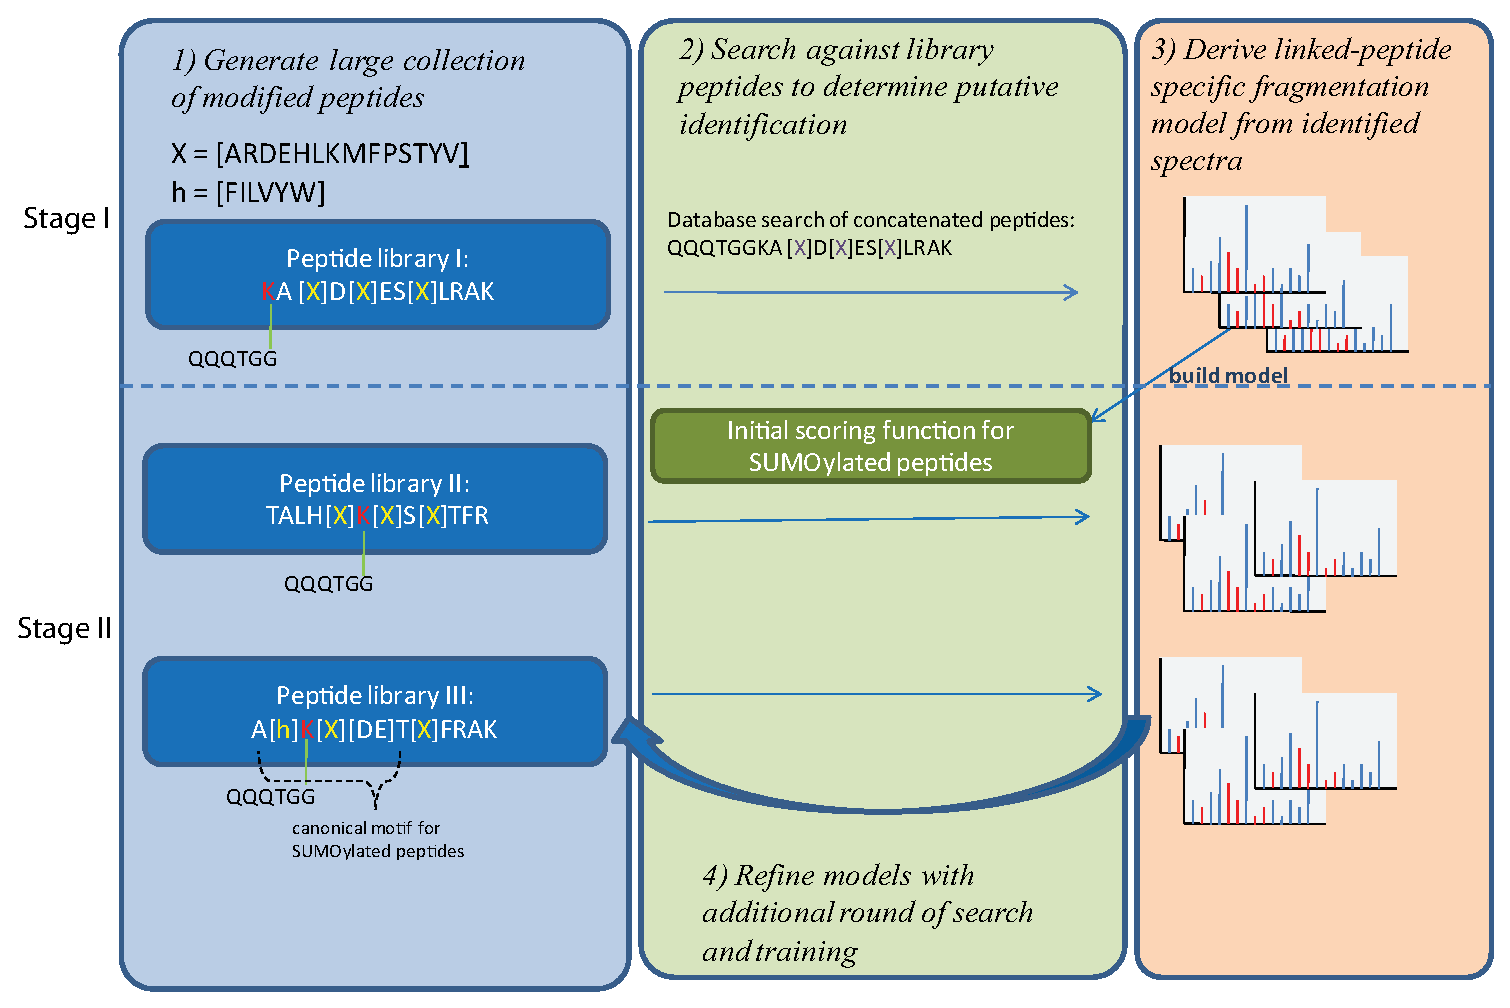
\includegraphics[height=100mm, width=150mm]{TRD4figures/Sumo_library_construction}
		\caption{{\bf Generating training data for linked peptides using combinatorial synthetic peptide libraries.} {\footnotesize In order to generate a large training dataset for SUMOylated peptides we designed and synthesized three combinatorial peptide libraries, each with a SUMO tag (QQQTGG) attached via a Lysine residue at a different position along the library peptide {\em (step 1)}. The sequence pattern for each library is shown on the left.  The symbols $X$ and $h$ stand for variable positions where multiple amino acid residues are possible, as indicated in the upper left corner.  Spectra from these peptide libraries are identified using a two-stage search strategy.  For library $I$, the SUMO tag is attached to the library peptide at the first residue.  Conceptually this is nearly equivalent to the substrate peptides having a prefix extension of QQQTGG. But since the SUMO tag is attached to the N-term Lysine and not to the N-term itself, the peptide fragmentation patterns are already expected to represent those of endogenous linked peptides with a similar structure of near-N-term linkage. We can identify spectra from library $I$ by searching a custom database where the sequence QQQTGG is concatenated to N-term of every possible peptide sequence in library $I$, thus allowing us to identify an initial set of spectra from SUMOylated peptides {\em (step 2)}. From this set we built a database search method specifically for SUMOylated peptides {\em (step 3)} and used it to identify spectra from peptide libraries $II$ and $III$ which are more realistic representations of SUMOylated peptides seen in biological samples (e.g., library $III$ encodes the canonical SUMO motif). Identified spectra from libraries $II$ and $III$ were then incorporated into the training set to build a more general scoring model for SUMOylated peptides {\em (step 4)}. Finally, we use the improved method to search the spectra from all three libraries once again to identify a final set of  spectra from SUMOylated peptides.}}
\label{librarybuild}
\end{figure}

A similar approach (illustrated in Figure~\ref{librarybuild})  was used to generate training data for disulfide-bridged peptides, except that in the initial round of searching (step 2 in Figure~\ref{librarybuild}) we used the scoring function learned from SUMOylated peptides. The sequence patterns used for the disulfide peptide libraries were: $I)$ \mbox{K[AW][DE]F[VSHY]A[DY]SCVA[KR]}, $II)$ \mbox{[TW]A[LE]H[FV]SCVT[PSGY]F[KR]} and
$III)$ \mbox{[WA]VK[FL]C[DE]T[VSGY]FA[KR]}. In theory this approach can be used to generate data for cross-linked peptides with any cross-linkers. However, during our initial testing, we found that the yield of cross-linked peptides from peptides libraries is quite low (only a few percentage of peptides form dimers), possibly due to the fact that peptides in solution are relatively far apart and the cross-linkers got hydrolyzed before they can react with the peptides.  We will address this issue by generating cross-linked peptides using disulfide-bridged peptides as a scaffold. After peptides in the library form disulfide-bridges and thus become spatially close to each other, we will $i)$ add cross-linkers to the dimers and $ii)$ reduce the disulfide bonds to create cross-linked peptides. Using this procedure we expect to be able to efficiently generate training data for cross-linked peptides with any available crosslinkers.

% After synthesis the peptide libraries were put in condition to promote the formation of random disulfide-bridged dimers.

\subsubsection{ Probabilistic fragmentation models for linked peptides}

We model an LPSM between a linked peptide $(P,Q)$ and a spectrum $S$ as a mixture of two PSMs $(P^*,S)$ and $(Q^*,S)$ 
%A match between a linked peptide pair and an MS/MS spectrum is modeled as a mixture of two peptides,
with each of peptides $P$ and $Q$ carrying a modification (modified peptides are denoted as $P^*$ and $Q^*$) 
at the cross-linked residue with mass equal to the mass of the linker plus the mass of the other peptide (Figure~\ref{linkedmodel}). 
%In regular database search for unlinked peptides, one evaluates how well a \emph{single} candidate peptide matches to a %given MS/MS spectrum. For crosslinked peptides we evaluate how well a \emph{pair} of peptides matches to a given MS/MS %spectrum.  
The universal probabilistic scoring models used for linked peptides is similar to that described in UniQuest (see Aim 1).  We will extend this model to further describe the fragmentation of a pair of peptides and also the specific fragmentation of linked fragment ions. 
%Similar to UniQuest, we aim to develop universal probabilistic models for linked peptides.

Briefly, an MS/MS spectrum is represented as a spectral vector 
%of $n$ bins, each representing a mass interval of width $\delta$ Da ($\delta$ depends on instrument resolution).  An %experimental MS/MS spectrum is represented as a vector 
$S = s_{1}, s_{2}, ... s_{n}$ where $s_{i}$ represents the peak intensity rank (ranked from most to least intense) of the highest-intensity peak in each bin.  Similarly, a theoretical spectrum of a peptide $P = p_{1}, p_{2}, ... p_{n}$ is represented as a peptide vector (see Aim 1).
%where $p_{i}$ indicates the ion-type of the fragment ion (e.g. b-ion or y-ion) with mass in that bin.  
The model captures peptide fragmentation statistics by using a set LPSMs  to learn the probability that each type of ion generates an observed peak with a given rank: $Prob(s|p)$.  Similarly a noise $Prob(s|0)$ model can be learned using unmatched peaks in the spectrum (where the symbol $0$ represents noise). In UniQuest, the scoring function for a PSM is defined as likelihood ratio of the probability that the spectrum $S$ is generated from the candidate peptide $P$ versus the probability that the  spectrum is generated from noise: $Score(S,P)=\sum{Score(s_{i}}, p_{i})=\sum{log(\frac{Prob(s_{i}|p_{i})}{Prob(s_{i}|0)})}$. Since linked peptides are represented as pairs of peptides, we represent a linked peptide as a pair of peptide  vectors $(P, Q)$. The vector $P = p_{1}, p_{2}, ... p_{n}$ contains all possible fragment ions from the first peptide while the vector $Q = q_{1}, q_{2}, ... q_{n}$ contains all possible fragments ions from the second peptide.  We define the first peptide to be the dominant peptide that accounts for more ion intensity in the spectrum.  This way we can account for possible differences in fragmentation patterns between the first and second peptides.  The score of an LPSM (P,Q,S)  is thus: $Score((P,Q),S) = \sum_i{\max(Score(s_{i}|p_{i}), Score(s_{i}|q_{i}))}$, where $\max$ is used to model the dependency between the two peptides. When theoretical fragment ions from both $P$ and $Q$ match to the same  spectrum peak, the model only uses the fragment ion with higher probability, thus avoiding using the same peak twice to support the identification of linked peptides. If not explicitly prevented, such double-counting will incorrectly bias unusually high scores towards pairs of peptide candidates sharing many of their theoretical fragment ions.

In order to capture the fragmentation statistics of crosslinked peptides, we further divide the set of fragment ion types into linked and non-linked fragments (Figure~\ref{linkedmodel}). Linked fragments are fragment ions that are covalently linked to a second peptide.  Thus for every ion type that is used to describe linear peptides we introduce its corresponding linked ion type in our probabilistic models.  For example, we will consider the ion types:  $b, b(iso), b-H2O, b-NH3, y, y(iso), y-H20, y-NH3$ for linear peptides, where $b(iso)$ indicates the first $^{13}C$ isotopic peak of a b-ion. Then we add the ion types $b_{X}, b(iso)_{X}, b-H2O_{X}, b-NH3_{X}, y_{X}, y(iso)_{X}, y-H2O_{X}, y-NH3_{X}$ to represent the corresponding linked-fragment ions that can be generated from linked peptides. For each ion type we consider charge states from one to the precursor charge of the  spectrum.  With these new ion types, the fragmentation statistics specific to linked peptide fragments will be learned during training and different probability/weights are assigned to linked and non-linked fragment ions.  In the full implementation of UniLink (as in UniQuest) we will make no special assumption about the ion types presented \-- all the ion types will be learned from the training data.

\subsubsection{Efficient database search for linked peptides}

We propose a two-step search strategy to avoid the quadratic search space of all possible linked peptides.  Since we model linked peptides as a pair of modified peptides, 
%, each with a modification at the linking site, 
we argue that for a linked peptide pair generating the  spectrum, at least one peptide should score reasonably well when matched to the spectrum alone. Thus in the first stage of our search we will match every peptide candidate against the query spectrum and sort them by their match score.  In the second stage only the top scoring peptides are then paired with the remaining candidates to find the best-scoring linked peptide pairs.  

Specifically, let $S$ be a query spectrum with parent mass $M_{S}$, $P$ be a peptide with parent mass $M_{P}$ and 
${P_{1}, P_{2}, ...... P_{n}}$ be a database containing $n$ peptides. A modified peptide $P(\Delta,t$ is  peptide $P$ with a mass-offset of $\Delta$~Da at the $t$-th amino acid residue. For each peptide $P_{i}$ in the database we consider all of its modified variants $P^m(\Delta,t)$, where $\Delta$ is the mass difference between the mass of the  spectrum and the mass of the candidate peptide:  $\Delta = M_{S} - M_{P_{i}}\ \  s.t. \Delta > 0$ and $t$ is all valid linking sites for the candidate peptide $P_{i}$. For example, in the case of disulfide-bridged peptides, all cysteine residue positions are considered. We score all of these modified candidate peptides against the query spectrum $S$ and sort all the peptide candidates according to their match score. In our training data, we found that in $approx 96\%$ of cases one of the linked peptides ranked 50 or less when searching against the library sequences appended to a large database of random (decoy) linked peptides.  Thus, rather than considering all possible peptide pairs, we take each of the top 50 peptide candidates and pair it with the remaining candidates in the database (such that their combined masses match the precursor mass of the  MS/MS spectrum) to find the best-scoring linked peptide pair in the database.

%With a new scoring function that are able to capture the specific fragmentation of linked peptides, we've demonstrated that it is able to improve our sensitivity of identifying linked peptides.  Conceptually, with our new scoring several techniques that has been used to improve the identification of single-peptide spectrum can seemlessly extended for the identification of linked peptides.  One such technique is tag-based filtering.  Note that although in 
UniLink avoids searching all possible linked peptide pairs by using the two-stage search strategy described above.  However, since the first stage is essentially a blind modification search, UniLink needs to consider almost every peptide candidate in the database.  This search space is considerably larger than regular database search of single-peptide spectra where one can filter the peptide candidates using parent mass filters. We will use tag-based filtering to substantially speed up regular~\cite{unv}{tanner05} and blind~\cite{unv}{na11} modification search of regular unlinked peptides. This stagging approach 
%A similar strategy can be used for linked peptides by $i)$ using an appropriate peptide fragmentation model and $ii)$ 
will require an extension of the  tagging algorithms developed at CCMS~\cite{tanner05,jeong2011} to process spectra of linked peptides (e.g., sequence tags may need to span multiple fragment ion charge states).
%except that the scoring function that evaluate how likely a sequence-tag can be generated from the  spectrum needed to updated to our new scoring function that properly captuer the fragmentation pattern of linked peptides.

\subsubsection{Evaluating statistical significance of LPSMs}



The generating function approach (MS-GF~\cite{unv}{kim08}) 
%introduced by CCMS to compute the statistical significance for PSMs
 was shown to greatly improve identification of unlinked peptides.  We propose to extend this concept for linked peptides by introducing two modifications to the original MS-GF approach. First, an MS-GF-compatible scoring function for linked peptides is required. Since the MS-GF approach is applicable with any additive scoring function, we expect that the probabilistic models described above will be  integrated into the MS-GF framework.  Second, we need to extend the MS-GF approach to the two-peptide case since a linked peptide spectrum is modeled as spectrum of two modified peptides. This extension is loosely related to the MS-GF extension proposed in TRD7 for identification of multiplexed spectra from co-fragmentation of multiple co-eluting precursor peptides.


\subsubsection{Preliminary results}

We implemented a pilot version of UniLink and tested its performance. We first evaluated the SUMO models on three different datasets. The first  dataset contain a set of synthetic SUMOylated peptides from the Human Myeloid cell leukemia protein (MCL1) spiked in a background of human cell lysate. The other two datasets are from published studies of endogenous SUMOylated peptides in Arabidopsis~\cite{unv}{miller2010proteomic} and Human~\cite{unv}{matic2010site}. 

Since currently there are no SUMO-specific peptide identification tools, the current practice is to search for them using via standard MS/MS database search tools allowing for a large PTM (our collaborators Drs. Gingras and Lill use Mascot and InsPecT).  
As shown in Figure~\ref{linkedIds}a, UniLink is able to identify significantly more 
%83\%--325\% more 
SUMOylated peptides than other tools.
%InsPecT or Mascot.
  Since we do not currently have datasets that contains disulfide-bridged peptides from biological samples, we tested our disulfide-bridged models on two datasets from crosslinking studies on S.~Pombe and on Rabbit proteasome using the crosslinker DSS~\cite{unv}{leitner2012expanding}.  Although it is suboptimal to not have DSS-specific fragmentation models, we assessed the performance of UniLink under the assumption that cross-linked peptides have fragmentation characteristics similar to disulfide-bridged peptides.  As shown in Figure~\ref{linkedIds}, UniLink is able to identify significantly more cross-linked peptides than the current state-of-the-art approach xQuest~\cite{unv}{rinner2008}. %{\tt Need a reference.} 

\begin{figure}[h!]
	\centering
		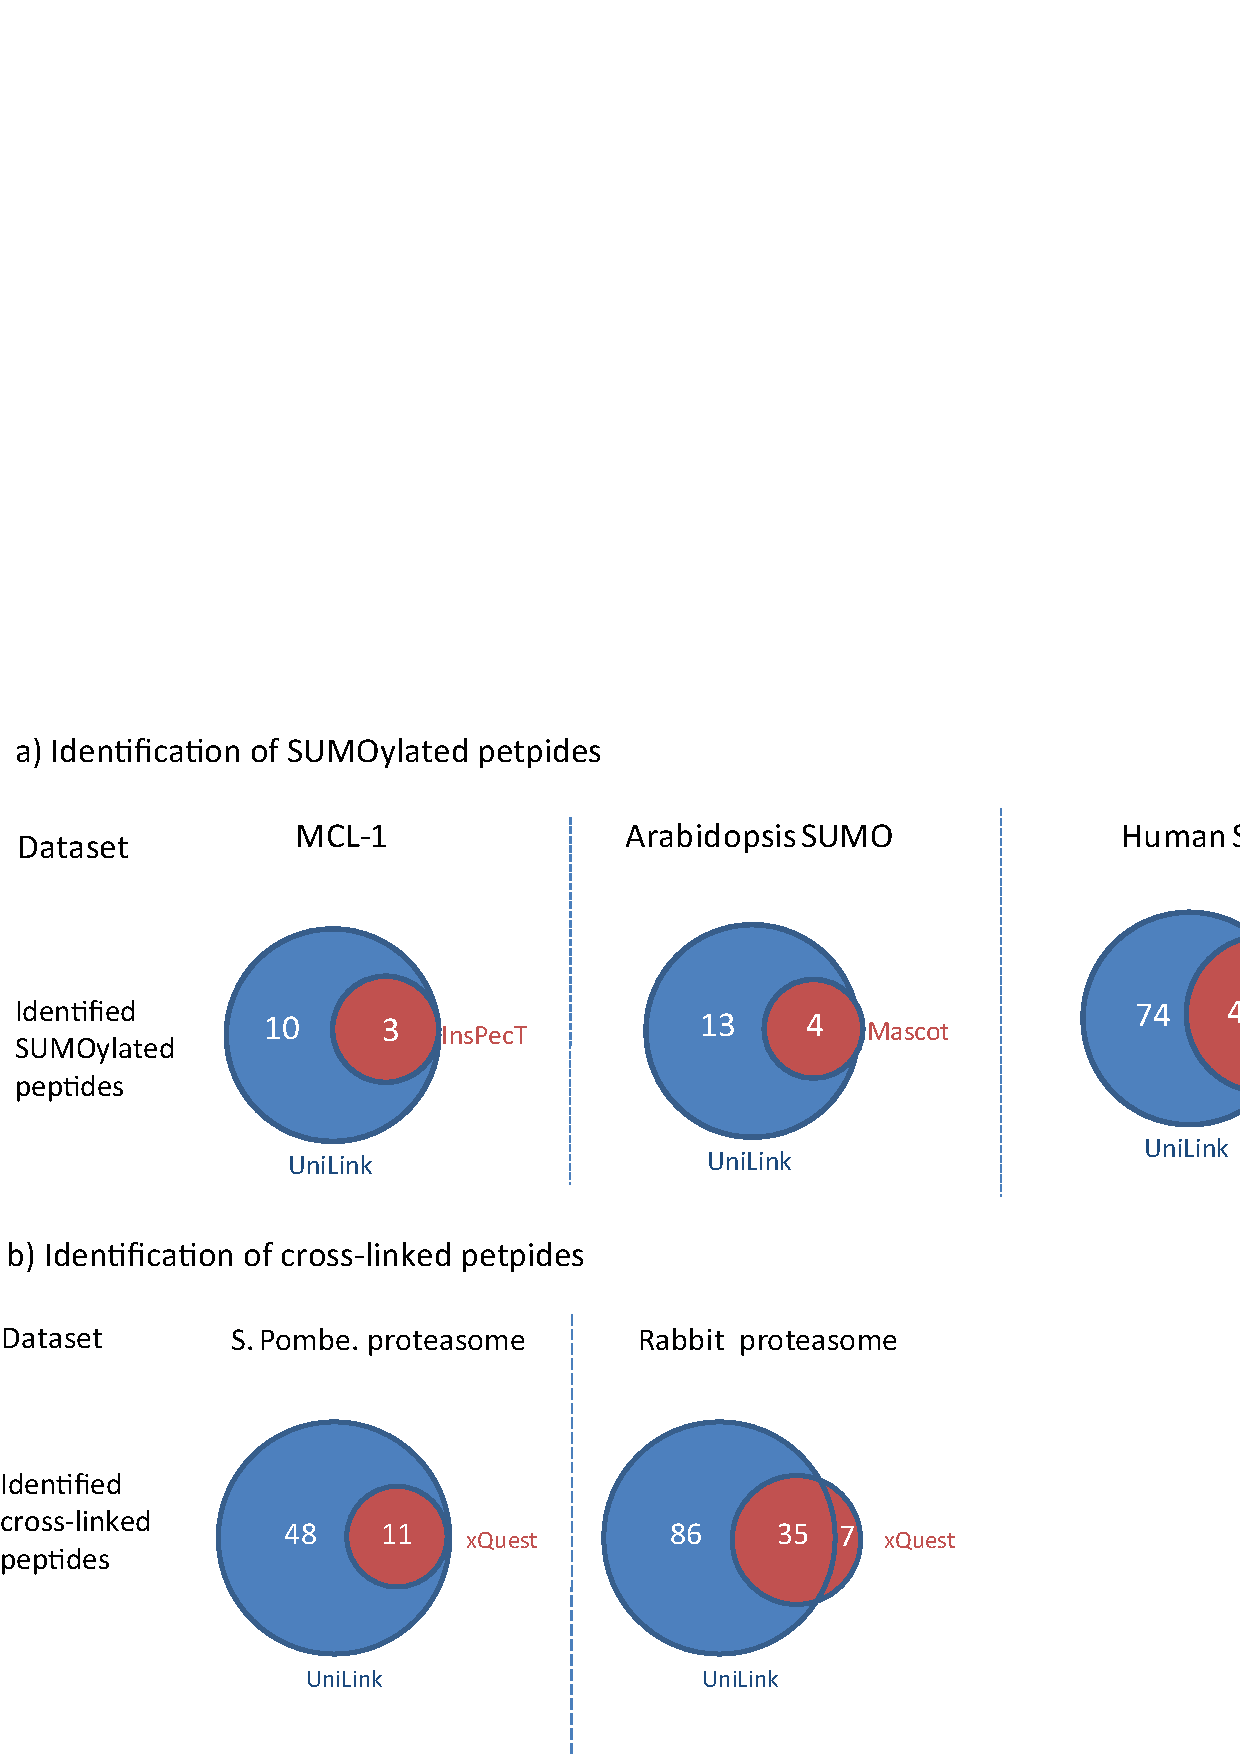
\includegraphics[height=100mm, width=150mm]{TRD4figures/linkedIDs_results.pdf}
		\caption{{\bf UniLink identification of linked
                    peptides.} {\footnotesize (a) The performance
                    of UniLink for identification of SUMOylated
                    peptides was tested in three datasets.  The MCL1
                    dataset contains 20 synthetic SUMOylated peptides
                    from MCL1 spiked in a background of human cell
                    lysate.  The
                    Arabidopsis~\cite{unv}{miller2010proteomic} and
                    Human SUMO~\cite{unv}{matic2010site} datasets were
                    reanalyzed from two previous proteomics studies
                    where identification of SUMOylated proteins and
                    peptides have been reported. UniLink significantly
                    improved the identification of SUMOylated
                    peptides.
                    (b) UniLink was tested on cross-linked
                    peptides using two datasets from crosslinking
                    studies on protein complexes: the S.Pombe 26S
                    proteasome and the Rabbit 20S
                    proteasome~\cite{unv}{leitner2012expanding}
                    (crosslinked with DSS). As shown UniLink
                    significantly improved the identification of
                    DDS-crosslinked peptides.}}
%UniLink is able to identify at least 288\% more crosslinked peptides than the current state-of-the-art tool xQuest.}}
\label{linkedIds}
\end{figure}

%{\tt Change MXDB into UniLink in the last Figure. Correct S.Pomes into S. Pombe. Correct petpides into peptides. Put a space after Rabbit} 

\subsection{Summary}


Many efforts have been invested into making peptide identification and sequencing  tools compatible with new types of data. 
For example, several pre-processing and post-processing strategies~\cite{unv}{Sweet:2009p12600,Hsieh:2009p12894} as well as several 
statistical modeling tools (e.g., PeptideProphet~\cite{unv}{Keller:2002p2677}
%DTASelect~\cite{unv}{Perkins:1999p6500} 
and Percolator~\cite{unv}{Kall:2007p10433}) have been proposed to boost the performance of  MS/MS database search tools. 
These tools do not find new PSMs,
but rather re-score PSMs reported by a database search tool using more complex scoring
and output high-scoring PSMs.
While they often improve  the
performance of a database search tool,  their performance
is negatively affected when the database search tool fails to find correct PSMs~\cite{unv}{Kim:2010p13586}. 
%For example, for spectra of Lys-N digests with non-standard fragmentation propensities, Mascot+Percolator (i.e., PSMs reported by Mascot and re-scored by Percolator) identifies only about half of the spectra compared to a database search tool equipped  with a dedicated scoring model for Lys-N~\cite{unv}{Kim:2010p13586}.
Another downside of the pre- or post-processing strategies
and statistical modeling tools is that since they are often not
integrated into database search tools, using them complicates the
analysis of MS/MS spectra. Our goal is to develop a tool that does not require any additional pre-processing, post-processing, or statistical modeling tools and thus makes the MS/MS analysis reproducible across different datasets and laboratories.  





Our preliminary analysis showed that for diverse types of spectral datasets, even the pilot versions of our universal tool identified more PSMs (and LPSMs)  than the state-of-the-art tools. In particular, UniQuest identified more PSMs that other peptide identification tools even when they are coupled with powerful 
 statistical modeling tools like  Percolator.
In fact, MS-GF+ has similar discriminating power as the leading spectral library search tool SpectraST~\cite{unv}{Lam:2007p6659}.
%
%The comparable performance of MS-GF+ and SpectraST indicates that access to previously identified spectra does not %necessarily translate into significant improvement in accurate peptide identification. 
It implies that scoring methods that compare Spectrum-Spectrum Matches (SSMs) are also important (see TRD3 for CCMS efforts to improve spectral library searches).  
In contrast to the sophisticated methods for PSM scoring used in database searches,
the library SSM scoring has not matured enough and is largely based on simple spectral cosine scores rather than statistical significance.
%We emphasize that  the generating function approach for accurately computing E-values significantly contributes to the improved performance of %MS-GF+.
%For example, when E-values instead of MS-GF scores were used to cut-off the results, 
%the number of identified PSMs increased approximately by 70\%, 50\%, and 20\% for LL, HL, and HH spectra, respectively.
In the new cycle, CCMS will improve the performance of spectral library search  by developing rigorous methods for computing statistical significance of SSMs (TRD3).

%Recently, many methods have been proposed to improve and 
%
%State-of-the-art statistical modeling tools like Percolator and PeptideProphet use semi-supervised classification algorithms to discriminate correct and incorrect PSMs
%using multiple scores reported by a database search tool (e.g. Xcorr, Sp, and delCn for SEQUEST).
%
%algorithms combine multiple scores reported by a database search tool af use multiple score The spectral E-values reported by MS-GF+ is just a single score 
%
%type of State-of-the-art analysis methods for interpreting MS/MS spectra are semi-supervised algorithms (PeptideProphet, Percolator, Gygi's LDA). 
%Most of them are based on old search engines. If MS-GF+ is used instead, the performance may improve.
%Example: Noble's recent paper to directly optimize the number of protein identifications.Lots of efforts have been made to post-process popular database search engines Mascot and Sequest.
%MS-GF+ outputs
%One can develop a post-processing method using the output of MS-GF+.
%Design post-processing methods (PTM localization) based on MS-GF+.

%We demonstrated that even a pilot universal {\em de novo} sequencing tool works well for diverse types of spectra. 
%UniNovo can be easily trained for different types of spectra using only thousands of PSMs. The prelimiary results show that UniNovo %generates accurate and long {\em de novo} reconstructions from spectra of CID, ETD, HCD, and CID/ETD fragmentation methods %and spectra of trypsin, LysC, or AspN digested peptides. We also showed that UniNovo is better than or comparable to other state of %the art tools. 

%Although UniNovo is developed as an automated  tool for high-throughput {\em de novo} sequencing, it also report the  spectrum logo that can be used for low throughput manual interpretation of spectra.  With UniNovo's reliable ion type prediction of peaks, the  spectrum logo enables the utilization of low intensity peaks that are however important.

As pointed out by \cite{unv}{ma11}, {\em de novo} sequences not only are valuable for the analysis of the novel peptides that are not present in proteome databases but also for various downstrean application like MS/MS database searches. 
%can facilitate the homology-based database searches. 
 Since UniNovo reports  
%representing the total mass of multiple amino acids 
gapped peptides~\cite{unv}{kim09_2,jeong11}) and  MS-BPM algorithm developed at CCMS~\cite{unv}{ng11} takes gapped peptides as an input, we will use  UniNovo$\oplus$MS-BPM for peptide identification.  
%MS-BPM enables searches against a sequence database using gapped peptides as queries. Currently MS-BPM takes gapped %peptides generated by MS-GappedDictionary~\cite{unv}{jeong11}. However, the reconstructions from UniNovo are usually longer %than those from MS-GappedDictionary (8-9 vs. 5-6).
 Since the search time of MS-BPM strongly depends on the length of gapped peptides (the longer gapped peptides, the faster is MS-BPM) and since UniNovo generates rather long peptides, UniNovo$\oplus$MS-BPM will result in an  extremely fast blind database search. This illustrates the synergy between CCMS efforts in peptide identification and de novo sequencing.  


\section{Driving Biomedical Projects}



%\bibliographystyle{plain}
%\bibliographystyle{ieeetr}
\bibliographystyle{unv}{ieeetr}

%\bibliographystyle{splncs}
%\bibliography{msgfplus,mybib,bandeiraLab,linked_msms,msms}
\bibliography{unv}{bibfiles/msgfplus,bibfiles/mybib,bibfiles/bandeiraLab,bibfiles/linked_msms,bibfiles/msms}{Literature Cited}


